% =====================================================================
%  Model lineage: from an 8-head mixture-density MLP to a contained,
%  stimulus-tuned, autoregressive-kinematics trajectory model.
%
%  Self-contained: no external figures, no \input. Upload this one file
%  to Overleaf and compile with pdfLaTeX (twice, for the ToC/refs).
% =====================================================================
\documentclass[11pt,a4paper]{article}

\usepackage[T1]{fontenc}
\usepackage[utf8]{inputenc}
\usepackage[margin=2.4cm]{geometry}
\usepackage{amsmath,amssymb}
\usepackage{booktabs}
\usepackage{array}
\usepackage{xcolor}
\usepackage{tcolorbox}
\usepackage{graphicx}
\usepackage{tikz}
\usepackage{pgfplots}
\pgfplotsset{compat=1.17}
\usetikzlibrary{arrows.meta,positioning,fit,backgrounds,calc}
\usepackage[colorlinks=true,linkcolor=blue!55!black,citecolor=blue!55!black,
            urlcolor=blue!55!black]{hyperref}


% Long \texttt{} identifiers (kin\_var\_comp, dot\_dist\_bias\_late, ...) cannot be
% hyphenated and would otherwise run into the margin. Let TeX stretch interword
% space a little on the offending lines instead.
\setlength{\emergencystretch}{2.5em}

% ---- units --------------------------------------------------------------
% Deliberately NOT siunitx: the units here are trivial, and dropping the
% package removes an expl3 version dependency that broke a real compile.
% All three work in text and in math mode.
\newcommand{\unit}[1]{\ensuremath{\mathrm{#1}}}   % standalone unit
\newcommand{\uu}[1]{\ensuremath{\,\mathrm{#1}}}  % unit after a number
\newcommand{\dg}{\ensuremath{^\circ}}             % degrees

% ---- semantic colours -------------------------------------------------
\definecolor{winc}{RGB}{0,110,60}
\definecolor{losec}{RGB}{170,30,30}
\definecolor{nullc}{RGB}{120,120,120}
\newcommand{\win}[1]{\textcolor{winc}{\textbf{#1}}}
\newcommand{\lose}[1]{\textcolor{losec}{#1}}
\newcommand{\nul}[1]{\textcolor{nullc}{#1}}

% ---- take-away box ----------------------------------------------------
\newtcolorbox{takeaway}{
  colback=blue!4, colframe=blue!35, boxrule=0.6pt, arc=2pt,
  left=6pt, right=6pt, top=4pt, bottom=4pt, before skip=6pt, after skip=10pt}
\newtcolorbox{keybox}[1]{
  colback=black!3, colframe=black!45, boxrule=0.7pt, arc=2pt,
  title={#1}, fonttitle=\bfseries\small,
  left=6pt, right=6pt, top=4pt, bottom=4pt}

% ---- shorthands -------------------------------------------------------
\newcommand{\dth}{\ensuremath{\Delta\theta}}
\newcommand{\auc}{\textsc{auc}}
\newcommand{\ctst}{C2ST}
\newcommand{\code}[1]{\texttt{\small #1}}
\newcommand{\ttbf}[1]{\texttt{\small\bfseries #1}}

\title{\vspace{-1.2cm}\textbf{From an 8-head mixture density to a contained\\
       trajectory simulator}\\[4pt]
       \large A step-by-step record of every mechanism added to the
       zebrafish bout model,\\ its motivation, and what it measured}
\author{Arthur Pollet}
\date{\today}

\begin{document}
\maketitle
\vspace{-0.8cm}

\begin{keybox}{One-paragraph summary}
A feed-forward mixture-density network predicting the next bout's reorientation angle
was extended, over nine controlled experiments, into a closed-loop trajectory simulator
with a tuned stimulus representation, autoregressive kinematics, and physical
containment. Judged by a classifier two-sample test on 39-dimensional trajectory
windows, generated behaviour went from \auc\ $0.890$ to $\mathbf{0.760}$ against a
real-versus-real floor of $\mathbf{0.476}$ --- about \textbf{31\% of the closable gap}.
Five changes were adopted, three measured as clean nulls, and four measured
\emph{resolvedly worse}. The predictive likelihood moved by $0.008$ bits/bout across all
24 evaluated rows (16 distinct models), because almost every accepted change lives outside
the likelihood ---
which is simultaneously the programme's main result and its main methodological caveat
(\S\ref{sec:twoobjects}).
\end{keybox}

\tableofcontents
\newpage

% =====================================================================
\section{What this document is}
% =====================================================================

This is a lineage record. It starts at the base model the user asked to start from ---
a one-hidden-layer MLP emitting eight per-bout parameters of a three-component angle
mixture --- and walks forward through every mechanism added since, in the order they were
added. Each step is presented in the same four parts:

\begin{description}\itemsep2pt
\item[Motivation.] The measured defect. Never ``it seemed like a good idea'': every step
      in this document was preceded by a diagnostic that produced a number.
\item[Mechanism.] What was actually implemented, with the equation and the configuration
      flag that switches it on.
\item[Result.] The paired contrast against that experiment's own control, with the
      $t$ statistic and a verdict of \emph{resolved} or \emph{within noise}.
\item[Take-away.] One sentence, boxed.
\end{description}

Failures are included at the same level of detail as successes, in
\S\ref{sec:negatives}. There are more of them than of successes, and several were more
informative --- three of the four most expensive mistakes in the programme were
\emph{methodological}, not architectural, and they are documented so they are not
repeated.

Because every decision here was made by a metric, the metric is defined first
(\S\ref{sec:eval}), before any model.

\paragraph{Scope.} The record runs from the base model through the ninth experiment
(\code{conv}). Two further experiments (\code{mem}, \code{indiv}) were built after this
document's cut-off; they are named in \S\ref{sec:next} but their results are deliberately
not tabulated here.

% =====================================================================
\section{The assay and the data}\label{sec:assay}
% =====================================================================

\subsection{Paradigm}

Juvenile zebrafish (15--21 dpf), each isolated in its own 10\uu{cm} circular
Petri dish, arranged in a $3\times5$ grid so that \textbf{15 fish are recorded
simultaneously}. Filming is from above under infrared at 30\uu{fps}. The visual
stimulus is a group of black dots, 2\uu{mm} in diameter, projected from below
to simulate conspecifics: a \emph{virtual shoal}.

The design is \textbf{lateralised}: at the onset of each block the dot group is placed to
the left or the right \emph{relative to the fish's own centroid}, and thereafter follows a
pre-recorded open-loop trajectory. This is the \code{CLsemi} (semi-closed-loop)
protocol --- closed-loop in its initial placement, open-loop in its subsequent motion.
Two consequences matter downstream:

\begin{enumerate}\itemsep2pt
\item Because the dot track is pre-recorded and shared, dot trajectories are essentially
      uncorrelated with fish behaviour across fish. Teacher-forcing the stimulus during
      evaluation is therefore legitimate.
\item Because the shoal is \emph{placed} relative to the real fish at block onset, the
      fish-to-shoal distance early in a block is an initial condition, not behaviour.
      This one fact invalidates the naive version of five evaluation metrics; see
      \S\ref{sec:panel}.
\end{enumerate}

Blocks alternate 60\uu{s} of stimulus with 50\uu{s} of pause, after a
20\uu{min} habituation with no visual stimulation. Dots move within a
$2.5\times2.5$\,cm area and never come closer than 0.5\uu{cm} to the fish
centre.

\subsection{Condition grid}

Stimulus labels follow the grammar
\code{CLsemi1800\_g\{$N_L$\}-\{$N_R$\}\_s\{$v_L$\}-\{$v_R$\}}, where \code{1800} is the
presentation length in frames ($1800/30 = 60\uu{s}$). Sixteen stimulus conditions
plus \code{inter\_stim\_pause} occur in the data:

\begin{center}\small
\begin{tabular}{lll}
\toprule
& \textbf{group sizes $N$} & \textbf{speed} \\
\midrule
moving & $1,\,2,\,4,\,6,\,8$ & $3.5$ \\
static & $1,\,4,\,8$         & $0$   \\
\bottomrule
\end{tabular}
\end{center}

each on either side, hence $2\times(5+3)=16$. Every observed label is single-sided
(\code{g\{N\}-0} or \code{g0-\{N\}}); the two-sided case never occurs. Per-condition bout
counts range 2{,}103--2{,}991, so the design is well balanced. Fish~0 shows 190
alternating blocks (95 stimulus, 95 pause), and total bout-onset span is
10448.8\uu{s} $=174.1\uu{min}$ --- the ``174-minute stimulus programme''
that later becomes a realism target (\S\ref{sec:guards}).

\subsection{Bout segmentation}

Segmentation follows Le Goc et al.\ (2021, \emph{BMC Biology},
\href{https://doi.org/10.1186/s12915-021-01126-w}{doi:10.1186/s12915-021-01126-w}),
adapted from their 25\,fps parameters to 30\,fps:

\begin{enumerate}\itemsep1pt
\item Positions Gaussian-smoothed ($\sigma = 2$ frames) \emph{for detection only}.
\item Instantaneous speed, then a 3-frame centred rolling mean.
\item Peak detection with an adaptive per-segment threshold
      $\mathrm{thr} = \overline{v} + k\,\mathrm{sd}(v)$, $k=1$, and a
      0.4\uu{s} refractory period.
\item \textbf{Onset $=$ the speed trough preceding the peak}, not Le Goc's fixed
      80\uu{ms} lead. Two rest points give a cleaner net-travel baseline and
      a meaningful fish pose at which to define the stimulus bearing.
\item Displacement gate over $\pm0.5\uu{s}$: reject bouts below
      0.3\uu{mm} (wobble) or above 18\uu{mm} (tracking jumps).
\end{enumerate}

Kinematics are computed \emph{onset-to-onset on the raw, unsmoothed positions}. The
reorientation is $\dth_i = \mathrm{wrap}_\pi(\theta_i - \theta_{i-1})$, so the first and
last bout of each tracking segment are dropped. Trajectories are split only at tracking
gaps, deliberately \emph{not} at stimulus-block boundaries --- a bout whose reorientation
spans a pause$\to$stimulus transition is the fish turning toward newly appeared dots,
which is the signal of this assay.

\subsection{Resulting dataset}

\begin{center}\small
\begin{tabular}{lr@{\hspace{2.2em}}lr}
\toprule
bouts & 70{,}590 & median inter-bout interval & 1.233\uu{s} \\
fish  & 15 (3{,}129--6{,}686 each) & median travel & 15.03\uu{px} $=$ 4.10\uu{mm} \\
frame rate & 30\uu{fps} & median $|\dth|$ & 39.0\dg{} \\
scale & 3.67\uu{px/mm} & forward / left / right & $0.111$ / $0.440$ / $0.449$ \\
bouts with a stimulus & 40{,}048 (56.7\%) & bouts with a \emph{moving} stimulus & 25{,}673 (36.4\%) \\
\bottomrule
\end{tabular}
\end{center}

Only 11\% of bouts fall inside the $\pm10\dg$ forward band, so the
$\{F,L,R\}$ alphabet used by the symbolic track is strongly turn-dominated.

Per-bout geometry is attached post-hoc: \code{dist\_to\_border\_norm} from the
\emph{true} physical dish ROI (distinct from the shipped trajectory-derived ROI, whose
radius is each fish's own 99.5th-percentile excursion), and \code{dot\_dist\_px},
\code{dot\_cx}, \code{dot\_cy}, \code{dot\_prox} from the active-dot centroid. The
pipeline is \textbf{pixel-native} throughout; there is no per-dish millimetre rescaling.

% =====================================================================
\section{Evaluation, defined before the models}\label{sec:eval}
% =====================================================================

Every step in \S\ref{sec:lineage} was adopted or rejected by the machinery in this
section, so the machinery has to come first. It has three layers: a likelihood, a panel
of interpretable distances, and two classifier two-sample tests. A fourth layer --- the
\emph{guards} in \S\ref{sec:guards} --- exists only because the third layer twice
rewarded a change that made the model worse in a way nothing was measuring.

\subsection{Cross-validation and the unit of analysis}

Folds are \textbf{leave-3-fish-out, 5 folds}, so each of the 15 fish is tested exactly
once and every comparison collapses to 15 paired per-fish scores. Everything that could
leak --- the inter-bout-interval and travel-distance pools used by generators, feature
standardisation scales, baseline counts, and \emph{every calibration constant} in
\S\ref{sec:lineage} --- is computed on the training fold only. Models are constructed
fresh from zero-argument factories inside each fold, so nothing survives across folds.

Uncertainty is always \textbf{fish-level (cluster) bootstrap}, never bout-level: 10{,}000
resamples of the 15 per-fish values, 95\% percentile interval. The fish is the
exchangeable unit; treating bouts as independent would understate every interval by
roughly the square root of the per-fish bout count.

\subsection{Metric A --- predictive log-density of the turn angle}

\begin{equation}
\text{bits/bout} \;=\; -\frac{1}{n}\sum_{t=1}^{n}
   \log_2 p\bigl(\dth_t \,\big|\, \dth_{1:t-1},\, \text{stimulus}_t\bigr),
\end{equation}
with the density taken with respect to Lebesgue measure \emph{in degrees}. By the chain
rule this equals the held-out joint log-likelihood per bout, which is exactly the scaled
forward algorithm's $\overline{\log c_t}$, so hidden Markov models and autoregressive
networks are directly comparable on it. A secondary track converts the same predictive
emission into a proper 3-symbol PMF over $\{F,L,R\}$ by integrating each component over
the $\pm10\dg$ bins (Normal \textsc{cdf}, regularised incomplete Gamma), and
reports its cross-entropy as \code{symbol\_bits}.

\begin{takeaway}
\textbf{Only the turn channel enters the \emph{reported} likelihood.} Inter-bout interval
and travel distance are not scored by Metric~A: every generative adapter's \code{score()}
returns a density over \dth\ alone. This is an \textbf{adapter convention, not a harness
guarantee} --- the harness averages whatever array it finds under the \code{logdens} key
without checking its channel, its shape or its measure, so an adapter returning a joint
density would be reported as Metric~A without complaint. The convention matters because
the models in this document \emph{do} carry distance and interval heads, and those heads
are trained inside a joint three-channel likelihood (\S\ref{sec:joint}); \code{score()}
simply never calls them. That, plus the fact that almost every later change is
generation-time only, is why \code{bits\_per\_bout} spans just $0.0084$ across all 24
evaluated rows while the trajectory \auc\ moves by $0.16$.
\end{takeaway}

\subsection{Metric B --- the interpretable panel}\label{sec:panel}

Free-running rollouts with the stimulus teacher-forced, $R=12$ independent rollouts per
held-out fish, matched to that fish's real bout count. Every quantity is computed per
fish, then aggregated across fish --- bouts are never pooled as if independent. The panel
has 21 entries; the ones that carry the argument in \S\ref{sec:lineage} are:

\begin{center}\small
\begin{tabular}{lll}
\toprule
\textbf{metric} & \textbf{definition} & \textbf{units, target} \\
\midrule
\code{abs\_dtheta\_w1} & Wasserstein-1 on $|\dth|$ & deg, $\to 0$ \\
\code{dist\_w1}, \code{dt\_w1} & Wasserstein-1 on travel, interval & px / s, $\to 0$ \\
\code{acf\_l2} & RMS error of turn-sign autocorrelation, lags $1\!-\!12$ & $\to 0$ \\
\code{following\_gap} & error in $P(\mathrm{sign}\,\dth{} = \mathrm{sign}\,\phi) - 0.5$ & prob., $\to 0$ \\
\code{following\_gap\_h} & same, scored against the bearing the model \emph{actually saw} & prob., $\to 0$ \\
\code{dot\_dist\_bias\_late} & signed fish-to-shoal distance error, $\geq40\uu{s}$ into a block & px, $\to 0$ \\
\code{wall\_frac\_gap} & signed error in $P(r/R > 0.85)$ & fraction, $\to 0$ \\
\bottomrule
\end{tabular}
\end{center}

Two of these deserve their motivation stated, because both encode a mistake that was
made first and corrected afterwards.

\paragraph{Why \code{\_late}.} The rig places the shoal roughly 75\uu{px} from the
\emph{real} fish at each block onset. A free-running generated fish is about
134\uu{px} away at that instant --- which is simply the swapped-track null --- and a
60\uu{s} block cannot close that at 2--4\,px per bout. So the raw dot-distance
gap is about two-thirds initial-condition artefact: $+23.4$\,px measured over all bouts
versus $+8.8$\,px measured $\geq40\uu{s}$ into a block. \emph{Read the
\code{\_late} variants.}

\paragraph{Why \code{wall\_frac\_gap} is separate.} A model that hugs the dish wall also
sits systematically far from a centrally-placed shoal. Without an explicit occupancy
metric, that \emph{containment} defect is only visible through the dot-distance
metrics --- i.e.\ it gets misattributed to the stimulus model. Reported separately,
it becomes the largest single win in the programme (\S\ref{sec:contain}).

\subsection{The two classifier two-sample tests}\label{sec:c2st}

A random forest (200 trees) is trained to separate real from generated 60-bout
non-overlapping windows, under \textbf{GroupKFold by fish}, so the classifier is always
tested on a fish it has never seen. Real windows carry label 1. The reported statistic is
the mean held-out \textsc{roc-auc}: $0.5$ means indistinguishable, $1.0$ means trivially
detectable.

\begin{center}\small
\begin{tabular}{p{0.16\textwidth}p{0.10\textwidth}p{0.62\textwidth}}
\toprule
\textbf{test} & \textbf{dims} & \textbf{features} \\
\midrule
turn \ctst{} & 20 &
  symbol frequencies (3), $3\times3$ transition matrix (9), $|\dth|$ mean/sd/median/q90 (4),
  turn-sign autocorrelation at lags 1--3 (3), mean run length (1) \\
\addlinespace
trajectory \ctst{} & 39 &
  the 20 above, plus travel distance mean/sd/median/q90/acf$_1$ (5), interval
  mean/sd/median/q90/acf$_1$ (5), fish-to-shoal distance (5), and radial occupancy
  $r/R$ mean/median/q90/$P(>0.85)$ (4) \\
\bottomrule
\end{tabular}
\end{center}

The trajectory test is the headline number: it is the only one that sees step sizes,
timing, proximity and occupancy. The turn test is retained because it isolates the
channel Metric~A scores.

\paragraph{The floor is 0.476, not 0.5.}
A negative control relabels each fish's \emph{real} windows into two random halves and
runs the identical classifier. Both classes are then real windows from the same
distribution, so the \auc\ should be $\approx 0.5$. It measures
$\mathbf{0.4761}$ and, crucially, is identical across all nine experiments. \emph{Every
\auc\ in this document must be read against $0.476$.} A model at $0.760$ has closed
$(0.890-0.760)/(0.890-0.476) = 31\%$ of the closable gap, not $26\%$ of the distance to
$0.5$.

\paragraph{Replicates, and why not pooling.}
Rollout randomness alone gives the trajectory \auc\ a standard deviation of $0.0173$ at
$R=1$ --- so the standard error of a two-model \emph{difference} is $0.0245$, and a
single rollout cannot resolve anything below about $0.035$ \auc. The fix is to average
\textbf{eight balanced single-rollout \auc{} s}, which cuts the standard error as
$1/\sqrt{R}$ without touching the level. Pooling replicates into one oversized generated
class instead would make the generated class $R$ times larger than the real one, and the
resulting class imbalance \emph{shifts} the level --- measured $0.790 \to 0.822$ at
$R=4$.

\paragraph{Common random numbers and the paired contrast.}
Each rollout draws from a stream keyed by $(\text{seed},\ \text{fish},\ \text{replicate})$
and \emph{deliberately not} by model index. Replicate $r$ of model~A and replicate $r$ of
model~B therefore see the same draws, and the per-replicate difference
$d_r = \auc_A[r] - \auc_B[r]$ cancels the shared rollout noise. Every contrast in
\S\ref{sec:lineage} is that paired difference:
\begin{equation}
t = \frac{\bar d}{\mathrm{sd}(d)/\sqrt{n}}, \qquad n = 8,\qquad
t_{\mathrm{crit}} = 2.3646 \ \ (\text{two-sided}, 7\ \mathrm{df}).
\end{equation}
Excluding the model from the stream key is not a detail. When a single generator was
threaded through the whole run, adding or reordering a model changed every other model's
draws --- the same configuration scored $0.760$ in one run and $0.7946$ in another purely
from list composition.

\paragraph{Attribution.} Permutation importances (the drop in held-out \auc\ when one
feature is shuffled in the test fold) are used rather than impurity importances. Impurity
is measured on the training split and biased toward high-variance features: it reports
where the forest looked, not what made the samples detectable. The two disagree whenever
features are correlated, and these are --- they are moments of the same channels.

\subsection{The guards, and why they exist}\label{sec:guards}

Twice, a change improved the headline \auc\ while making the model materially less
realistic in a dimension nothing was measuring. Both times the instrument was built
afterwards. They are now reported on the same line as every \auc.

\paragraph{Dispersion.}
The \auc\ says \emph{how} detectable a model is; it cannot say whether the model is too
narrow or too wide, and those need opposite fixes. \code{dispersion\_report} gives two
numbers with unambiguous targets: per-group variance ratio
$\sum\mathrm{var}(\mathrm{gen}) / \sum\mathrm{var}(\mathrm{real})$ over real-$z$-scored
window features (target $1.0$; $<1$ under-dispersed, $>1$ over-dispersed), and the
\textbf{between-fish variance share} --- the fraction of total window variance carried by
the per-fish means (real: $\mathbf{0.2551}$). It was written because the \code{kin}
experiment won $-0.0407$ \auc\ while \emph{halving} generated distance dispersion, from
$1.04$ to $0.52$ against a target of $1.00$.

\paragraph{Timing and realism.}
\code{timing\_report} adds thirteen quantities the per-bout panel is blind to: the
time-weighted quiescent budget (fraction of \emph{elapsed time} in gaps
$>5/20/60\uu{s}$), the clock ratio $\sum \mathrm{d}t_{\mathrm{gen}} /
\sum \mathrm{d}t_{\mathrm{real}}$, the interval right-tail, the autocorrelation of bout
count per minute, the cross-channel couplings, the distance standard-deviation ratio, the
between-fish spread of turning style, and the containment-guardrail bounce rate. Real
reference values worth quoting:

\begin{center}\small
\begin{tabular}{ll}
\toprule
time in gaps $>20\uu{s}$ & \textbf{24.4\%} of the session, from only $\sim$0.6\% of bouts \\
bout-rate autocorrelation at 1/2/3\,min & $0.51$ / $0.33$ / $0.22$ \\
$\mathrm{corr}(\log \mathrm{d}t, \log \mathrm{dist})$ across windows & $-0.386$ \\
$\mathrm{corr}(\log \mathrm{d}t, |\dth|)$ across windows & $+0.308$ \\
between-fish sd of forward fraction & $0.054$ \\
between-fish sd of median $|\dth|$ & 6.73\dg{} \\
\bottomrule
\end{tabular}
\end{center}

It was written because the \code{conv} experiment won $-0.0113$ \auc\ while cutting
quiescent time from 13.0\% to \textbf{6.9\%} of the session against a real 24.4\%, and
finishing the 174-minute stimulus programme in 142 minutes.

\paragraph{Marginal equalisation.}
``The model gets levels wrong'' and ``the model gets within-fish temporal structure
wrong'' are different defects with different fixes, and the headline \auc\ cannot
separate them. \code{rank\_map} maps each generated channel onto the held-out fish's real
marginal \emph{by rank}, preserving order, so the residual \auc\ concerns temporal
structure alone. It is an oracle --- it uses held-out marginals --- so an equalised \auc\
is never a model score. Report both, never the equalised one alone.

\begin{takeaway}
The reading protocol is three numbers on one line: \textbf{\auc\ against the $0.476$
floor}, \textbf{the dispersion table}, and \textbf{the timing table}. Two accepted
changes in this document would have been rejected, or at least qualified, had the second
and third existed at the time.
\end{takeaway}

% =====================================================================
\section{The base model: an 8-head mixture density network}\label{sec:base}
% =====================================================================

\subsection{Emission family}

The angle emission is inherited unchanged from the project's hidden Markov models, which
is what makes the two families comparable on Metric~A:
\begin{align}
p(\dth) &= w_F\,\mathcal{N}(\dth;\,0,\sigma_F)
         + w_L\,\Gamma(-\dth;\,\alpha_L,\theta_L)\,\mathbf{1}[\dth<0] \nonumber\\
        &\qquad + w_R\,\Gamma(+\dth;\,\alpha_R,\theta_R)\,\mathbf{1}[\dth>0],
        \qquad \textstyle\sum w = 1 .
\end{align}
Three components: a forward mode centred at exactly zero, and one Gamma per turn
direction. The Normal mean is fixed at $0$ and is never a network output.

The network replaces the HMM's latent-state prior over $\{F,L,R\}$ with a direct
feed-forward function of recent history and stimulus. It is one hidden layer with ReLU,
and in the \code{'full'} variant --- the one this lineage starts from --- a linear head
producing \textbf{eight per-bout outputs}:

\begin{center}\small
\begin{tabular}{clll}
\toprule
\textbf{index} & \textbf{quantity} & \textbf{link} & \textbf{note} \\
\midrule
0,\,1,\,2 & $\log w_F,\ \log w_L,\ \log w_R$ & $\mathrm{log\_softmax}$ & mixture weights \\
3 & $\sigma_F$   & $\mathrm{softplus}+\varepsilon$ & forward width \\
4 & $\alpha_L$   & $\mathrm{softplus}+1$ & left shape \\
5 & $\theta_L$   & $\mathrm{softplus}+\varepsilon$ & left scale \\
6 & $\alpha_R$   & $\mathrm{softplus}+1$ & right shape \\
7 & $\theta_R$   & $\mathrm{softplus}+\varepsilon$ & right scale \\
\bottomrule
\end{tabular}
\end{center}

All eight vary per bout, so the model is heteroscedastic and the two Gammas are
asymmetric --- the left and right turn distributions may differ in both shape and scale.
(A simpler \code{'basic'} variant emits only the three weight logits and keeps
$\sigma,\alpha,\theta$ as global learnable scalars with a symmetric Gamma. It is not part
of this lineage.)

\subsection{Input features}

The feature matrix is assembled block-wise, and \emph{the column order is a contract}:
the closed-loop generators rebuild single rows of it from the generated pose, so any
drift between the two silently corrupts the rollout. Two blocks were later rewritten to
share one vectorised, scalar-safe function between training and generation precisely to
make that hazard structurally impossible.

\begin{center}\small
\begin{tabular}{llp{0.50\textwidth}}
\toprule
\textbf{block} & \textbf{dims} & \textbf{contents} \\
\midrule
history      & $K$ & previous $K$ reorientations, scaled by a train-fold standard deviation \\
stimulus     & $s$ & see \S\ref{sec:stim} --- from 1 to 21 channels depending on mode \\
border       & 3 or 9 & $[d_{\mathrm{norm}}, \sin\psi, \cos\psi]$, $\psi$ the egocentric bearing to the dish centre \\
adaptation   & 2 & $[\text{prox},\ \text{prox} - a]$ with $a$ a leaky integral of proximity \\
kinematic history & $2K_{\mathrm{kin}}$ & previous $z$-scored $\log$ travel and $\log$ interval \\
\bottomrule
\end{tabular}
\end{center}

so $D = K + s + b + 2\,[\text{adapt}] + 2K_{\mathrm{kin}}\,[\text{kin}]$. The models in
this document use $K=8$, hidden width 128, and the raw 3-channel border block unless
stated; the canonical configurations are therefore $D=14$ (\code{dotb}), $D=24$
(\code{shoalr}), $D=29$ (\code{shoal}).

The border block's rationale is worth stating because it recurs: distance to the wall
alone cannot say \emph{which way} to turn, so the sine and cosine of the inward bearing
supply the direction --- exactly analogous to the stimulus bearing.

\subsection{Training}

Objective is the mean negative log mixture density. Adam, learning rate $10^{-3}$, weight
decay $10^{-5}$, batch size 256, a random 15\% bout-level validation split for early
stopping (fish-level splitting happens outside, in the cross-validation), improvement
threshold $10^{-4}$, and the best state restored at the end.

\paragraph{Determinism.}
Two identical-configuration fits are bitwise identical on CPU --- the code has no RNG
leak --- but on an A100 the same configuration produced held-out $7.7388$ versus $7.7365$
bits/bout, which involves no sampling at all and is a pure function of the weights. That
fit-to-fit spread of $\sim0.003$ on the trajectory \auc\ is comparable to the $\sim0.005$
rollout standard error the paired contrast reports, and the paired-on-replicate contrast
treats the fitted model as \emph{fixed}, so it cannot see it. cuBLAS matmul reductions use
atomics unless a fixed workspace is configured; the fix is to set the workspace
environment variable before the first CUDA context, disable cuDNN benchmarking (which
autotunes per run and so picks different algorithms), and request deterministic
algorithms. \textbf{Without this, no effect below $\sim0.01$ \auc\ is resolvable.}

% =====================================================================
\section{First change: a five-component emission}\label{sec:mix}
% =====================================================================

\paragraph{Motivation.}
Permutation importances on the best three-component model put the residual detectability
on the \emph{turn-magnitude} features --- $|\dth|$ median, standard deviation, q90, mean.
A single Gamma per side cannot fit the body and the tail of a turn-magnitude distribution
at once.

\paragraph{Mechanism.}
Split each side into two Gammas: a short-turn and a long-turn component.
\begin{equation}
p(\dth) = w_F\,\mathcal{N}(0,\sigma_F)
 + \sum_{k=1}^{2} w_{Lk}\,\Gamma(-\dth;\alpha_{Lk},\theta_{Lk})
 + \sum_{k=1}^{2} w_{Rk}\,\Gamma(+\dth;\alpha_{Rk},\theta_{Rk}).
\end{equation}
The head grows from 8 to \textbf{14 outputs}: 5 weight logits, $\sigma_F$, and four
$(\alpha,\theta)$ pairs. \emph{Only the emission changes} --- the input features are
reused verbatim --- so this is a clean emission-only comparison, and the symbol PMF
integration generalises directly to two Gammas per side.

\begin{takeaway}
Everything from here on uses the 5-component emission. It is the last change in this
document to the \emph{turn emission family itself}; later changes still enter the fitted
model, but as input features, as separate kinematic heads, or as training budget.
\S\ref{sec:twoobjects} sorts them.
\end{takeaway}

% ---------------------------------------------------------------------
\subsection{What the baseline already contains --- including a joint
            likelihood}\label{sec:joint}
% ---------------------------------------------------------------------

Between the 8-head network of \S\ref{sec:base} and the first experiment of
\S\ref{sec:lineage} the model acquired four things that are \emph{not} attributable to any
ladder below, because they were already present in the very first control. Stating them
here prevents the lineage from taking credit for them:

\begin{enumerate}\itemsep2pt
\item the 5-component emission just described;
\item an \textbf{honest closed loop} --- the wall covariate \emph{and} the stimulus bearing
      are recomputed from the fish's own generated pose each bout, so a drifted fish sees
      the shoal where it actually is relative to itself;
\item a \textbf{separate kinematic trunk} (width 32) reading only the kinematic history
      block and feeding a log-normal travel-distance head and a log-normal interval head,
      the latter conditioned on the sampled log-distance;
\item the per-trajectory \code{vigor} latent.
\end{enumerate}

Item 3 changes what ``the likelihood'' means, and it is worth being explicit because the
rest of the document depends on the distinction. The network is trained by minimising a
\textbf{joint three-channel negative log-likelihood}:
\begin{equation}\label{eq:joint}
\mathcal{L} \;=\; -\Bigl[\;
  \underbrace{\log p(\dth \mid x_{\mathrm{ang}})}_{\text{5-component mixture}}
  \;+\; \underbrace{\log p(\ell \mid x_{\mathrm{kin}})}_{\text{log-normal, travel}}
  \;+\; \underbrace{\log p(\tau \mid x_{\mathrm{kin}}, \log \ell)}_{\text{log-normal, interval}}
\;\Bigr],
\end{equation}
with $\ell$ the travel distance and $\tau$ the inter-bout interval. The interval head takes
$\log \ell$ as an input, so the kinematic pair is a genuine joint density
$p(\ell,\tau) = p(\ell)\,p(\tau \mid \ell)$ rather than two independent marginals. The
angle is conditionally independent of both, since it sits on its own trunk.

\subsubsection*{What the three conditional densities actually are}

Each channel has a \textbf{fixed emission family whose parameters are per-bout network
outputs}. That is where the conditioning lives: the functional form never changes, and the
density function itself cannot see the features --- \code{mix\_logdens} takes no feature
argument at all. Writing $\mathcal{N}$ for the normal density and
$\Gamma(u;\alpha,\theta) = u^{\alpha-1}e^{-u/\theta}/(\theta^{\alpha}\Gamma(\alpha))$ for the
shape--scale Gamma on $u>0$, the turn channel is
\begin{equation}\label{eq:pang}
\begin{aligned}
p(\dth \mid x_{\mathrm{ang}}) \;=\;\;&
   w_F(x)\,\mathcal{N}\bigl(\dth;\,0,\sigma_F(x)\bigr) \\[2pt]
 &+\; \sum_{k=1}^{2} w_{Lk}(x)\,\Gamma\bigl(-\dth;\,\alpha_{Lk}(x),\theta_{Lk}(x)\bigr)
  \;+\; \sum_{k=1}^{2} w_{Rk}(x)\,\Gamma\bigl(+\dth;\,\alpha_{Rk}(x),\theta_{Rk}(x)\bigr),
\end{aligned}
\end{equation}
every argument written $(x)$ being a function of $x_{\mathrm{ang}}$ through the network.
The two kinematic channels are \textbf{mixtures of log-normals}. With
$\mathrm{LN}(x;\mu,\sigma) = \frac{1}{x\sigma\sqrt{2\pi}}
 \exp\!\bigl(-(\log x-\mu)^2/2\sigma^2\bigr)$,
\begin{align}
p(\ell \mid x_{\mathrm{kin}}) &= \sum_{k=1}^{n_{\mathrm{dist}}}
    w^{\ell}_k(x_{\mathrm{kin}})\;
    \mathrm{LN}\bigl(\ell;\,\mu_k(x_{\mathrm{kin}}),\,\sigma_k(x_{\mathrm{kin}})\bigr),
    \label{eq:pdist}\\[2pt]
p(\tau \mid x_{\mathrm{kin}}, \log\ell) &= \sum_{k=1}^{n_{\mathrm{dt}}}
    w^{\tau}_k(x_{\mathrm{kin}},\log\ell)\;
    \mathrm{LN}\bigl(\tau;\,m_k(x_{\mathrm{kin}},\log\ell),\,s_k(x_{\mathrm{kin}},\log\ell)\bigr).
    \label{eq:pdt}
\end{align}
After the \code{tail} experiment (\S\ref{sec:lineage}) $n_{\mathrm{dist}}=2$ and
$n_{\mathrm{dt}}=3$; before it they were 1 and 2, and the one-component case is
special-cased as a bare $(\mu,\sigma)$ pair with no weight.

\paragraph{Parameters and their links.} Every raw network output is mapped to a valid
parameter by one of three links. $\varepsilon = 10^{-12}$ is a numerical guard;
$\alpha_{\min} = 1$ is a \emph{modelling} constraint.

\begin{center}\small
\begin{tabular}{llll}
\toprule
\textbf{channel} & \textbf{raw outputs} & \textbf{quantity} & \textbf{link} \\
\midrule
turn        & 14 (one head on $x_{\mathrm{ang}}$)
            & 5 mixture weights & $\mathrm{log\_softmax}$ \\
            & & $\sigma_F$, four $\theta$ & $\mathrm{softplus}(\cdot)+\varepsilon$ \\
            & & four $\alpha$ & $\mathrm{softplus}(\cdot)+\alpha_{\min}$ \\
\addlinespace
travel      & $3n_{\mathrm{dist}}$ (kin trunk)
            & weights / $\mu$ / $\sigma$ &
              $\mathrm{log\_softmax}$ / identity / $\mathrm{softplus}+\varepsilon$ \\
\addlinespace
interval    & $3n_{\mathrm{dt}}$ (kin trunk $\oplus \log\ell$)
            & weights / $m$ / $s$ &
              $\mathrm{log\_softmax}$ / identity / $\mathrm{softplus}+\varepsilon$ \\
\bottomrule
\end{tabular}
\end{center}

The $\alpha \geq 1$ floor is not cosmetic: $\Gamma(u;\alpha,\theta) \sim u^{\alpha-1}$ as
$u \to 0^{+}$, so $\alpha < 1$ would let the density \emph{diverge} at zero turn angle.
With $\alpha > 1$ enforced, all four Gammas vanish there and \textbf{every bit of
probability mass near $\dth = 0$ comes from the forward Normal alone} --- which is what
makes the forward/turn decomposition identifiable.

\paragraph{The densities are over the raw observables, not their logarithms.} The
implemented kinematic log-densities lead with a $-\log x$ term. That is the
change-of-variables Jacobian, and it is what makes
Eqs.~\eqref{eq:pdist}--\eqref{eq:pdt} densities on pixels and seconds rather than Gaussians
on $\log$-pixels and $\log$-seconds. (Verified by numerical integration: the implemented
functions integrate to $1.000$ over the raw variable and to $0.089$ read as log-space
densities.) Only with the Jacobian present do the three terms compose into a genuine joint
density --- with respect to the product measure $\mathrm{deg} \times \mathrm{px} \times
\mathrm{s}$. One consequence to keep in mind: the terms are \emph{dimensional}, so their
magnitudes are not comparable with one another and shift by a constant under a change of
units (px\,$\to$\,mm moves the travel term by $\log 3.60$ per bout).

Three consequences run through everything that follows.

\begin{itemize}\itemsep3pt
\item \textbf{The reported likelihood is a strict subset of the fitted one.} Metric~A
      evaluates only the first term of Eq.~\eqref{eq:joint}. The other two are optimised
      and then never reported.
\item \textbf{The angle path is nevertheless coupled to the kinematic channels}, through
      exactly one route: early stopping. The three terms are additively separable and the
      two parameter groups are disjoint, so angle gradients are unaffected --- but the
      checkpoint that is kept is selected on the \emph{joint} validation loss, and the
      saved state is the full network. The turn density Metric~A scores is therefore chosen
      by a criterion that includes distance and timing.
\item \textbf{The three terms are averaged separately.} Each is a mean over its own
      finite-value mask before being summed, so the objective weights the channels equally
      regardless of how many bouts survive each mask. It coincides with a pooled joint NLL
      only when both kinematic masks are full.
\end{itemize}

% ---------------------------------------------------------------------
\subsection{Notation used from here on}\label{sec:notation}
% ---------------------------------------------------------------------

\begin{center}\small
\renewcommand{\arraystretch}{1.16}
\begin{tabular}{@{}>{$}l<{$}p{0.40\textwidth}p{0.36\textwidth}@{}}
\toprule
\textrm{\textbf{symbol}} & \textbf{meaning} & \textbf{units / range} \\
\midrule
\multicolumn{3}{@{}l}{\textit{observables (one per bout)}}\\
\dth      & signed reorientation angle & degrees, $(-180,180]$ \\
\ell      & travel distance to the next bout & px (3.67\uu{px/mm}) \\
\tau      & inter-bout interval & s \\
\midrule
\multicolumn{3}{@{}l}{\textit{stimulus geometry}}\\
\phi      & egocentric bearing to the active-dot centroid; $+$ is to the fish's left & rad \\
r         & fish-to-shoal centroid distance & px \\
N         & number of dots in the group & $\{1,2,4,6,8\}$ \\
\midrule
\multicolumn{3}{@{}l}{\textit{dish geometry}}\\
u         & radial position $\lVert\mathbf{p}-\mathbf{c}\rVert / R$ & $0$ = centre, $1$ = wall \\
d_{\mathrm{norm}} & distance to the wall, $=1-u$ & $0$ = wall, $1$ = centre \\
\psi      & egocentric bearing to the dish centre & rad \\
R         & physical dish radius & $\approx$\,176\uu{px} \\
\midrule
\multicolumn{3}{@{}l}{\textit{the range basis (\S\ref{sec:stim})}}\\
c_j       & \textbf{knot} --- a reference distance at which one basis function peaks &
            $(25,50,90,160)$\,px \\
\hat g_j  & softmax basis weight at range $r$; $\sum_j \hat g_j = 1$ & dimensionless \\
w         & basis width & $0.40$ natural-log units \\
n_z       & normalised group size, $\log_2 N/\log_2 8$ & $[0,1]$ \\
r_z       & signed log-range, $\mathrm{clip}((\log r-\log 70)/\log 4,-1,1)$ &
            $\pm1$ = $\pm2$ octaves \\
\midrule
\multicolumn{3}{@{}l}{\textit{calibrated constants}}\\
\lambda   & kinematic feedback shrinkage (\S\ref{sec:kin}) & $(0,1]$, $1$ = no shrinkage \\
u_0       & shell gate threshold (\S\ref{sec:contain}) & $0.75$ in $u$ \\
s         & containment bias scale & $(\mathrm{bulk},\mathrm{shell}) = s\cdot(4^\circ,35^\circ)$ \\
W         & analysis window & 60 bouts, non-overlapping \\
K         & turn-history lags in $x_{\mathrm{ang}}$ & 8 \\
K_{\mathrm{kin}} & kinematic-history lags in $x_{\mathrm{kin}}$ & 3 \\
n_{\mathrm{dist}}, n_{\mathrm{dt}} & log-normal components on the travel / interval head &
            $1,2 \to 2,3$ after \code{tail} \\
\bottomrule
\end{tabular}
\end{center}

\noindent\small A \textbf{knot} is nothing more than a reference distance: each basis
function $\hat g_j$ is a bump centred on its knot $c_j$, the network learns one turning
gain per knot, and the response at any range is the softmax-weighted blend. The notebook
plots the four basis functions directly, which is the quickest way to see it.\normalsize

% =====================================================================
\section{The lineage, experiment by experiment}\label{sec:lineage}
% =====================================================================

Nine experiments were run, each as a ``ladder'': a control plus one to three variants,
all fitted and evaluated inside a single run under common random numbers, so the paired
contrast is valid. Protocol was identical throughout: 5 folds, $R=12$ rollouts, 8
\ctst\ replicates, 80 training epochs, seed 0.

\begin{keybox}{Where the numbers come from --- and two different kinds of them}
Every quantitative claim in this section is re-derived, with its plot and the code that
produced it, in \code{notebooks/model\_lineage\_walkthrough.ipynb}. Each subsection carries
a \emph{How this was measured} paragraph naming the estimator, the window and how many fish.

\medskip
\textbf{The two kinds are not interchangeable, and this document previously blurred them.}

\emph{Cross-validated.} Every \auc, $\Delta$, $t$ and Metric-B panel value comes from
\code{quick\_results}: leave-3-fish-out over 5 folds, so each fish is scored by a model that
never saw it. \textbf{These are the numbers the lineage was decided on.}

\emph{In-sample.} The \code{.pt} checkpoints on disk are a \emph{separate}, later fit on
\textbf{all 15 fish}, made explicitly ``for local diagnostics'' so that range- and
wall-resolved profiles could be run without a GPU. Anything obtained by rolling one of them
out --- the range profile, the entry/dwell decomposition, the guardrail forensics, the tail
quantiles, the quiescent budget --- is therefore \emph{in-sample}. Those quantities describe
\emph{a} fitted model faithfully and are the right tool for asking ``what does this mechanism
do'', but they are not held-out performance and no ladder decision rests on them.
\end{keybox}

\begin{keybox}{A comparison rule that is easy to violate}
\textbf{Absolute \auc\ values are not comparable across experiments.} Each ladder refits
its own control, and refits differ: the identical model \code{contain\_tail} reads
$0.7714$, $0.7681$, $0.7712$ and $0.7712$ in four different ladders. Only the
\emph{within-ladder paired delta} is a measurement. Absolute values below are context,
not evidence.
\end{keybox}

% ---------------------------------------------------------------------
\subsection{\texttt{stim} --- the \emph{turn response} was blind to range}\label{sec:stim}
% ---------------------------------------------------------------------

\paragraph{Motivation.}
The baseline stimulus representation was \code{dotb}: $[\sin\phi, \cos\phi,
\text{moving}]$, a pure bearing. Two range-resolved diagnostics show what is missing.

\emph{Turning.} $P(\text{turn toward the shoal})$ per range bin is an
\textbf{inverted-U}: real fish measure $0.549$ at $r<25$\,px, rising to $0.656$ at
70--90\,px, then falling back to $0.585$ beyond 120\,px. Curvature (peak bin minus the mean
of the two end bins) is $+0.090$ for real fish and $-0.009$ for \code{dotb} --- i.e.\ the
bearing-only model is \emph{flat}.

\emph{Closing.} The restoring force $E[\Delta r \mid r]$ crosses zero at
41.4\uu{px}: inside that radius the fish is on average \emph{increasing} its distance
from the shoal. This is the quantity that changes sign at close range --- not
$P(\text{turn toward})$, which stays above $0.5$ in every bin. An earlier version of this
document conflated the two.

A monotone proximity weight of the form $1/(1+r/r_0)$ --- which is what the alternative
\code{dot} mode used --- can represent neither a peak nor a sign change.

\paragraph{How this was measured.}
\code{diag\_range\_profile.\_profiles}, on \textbf{moving-dot bouts only}, binned by
fish-to-shoal centroid distance with edges $(0,25,40,55,70,90,120,\infty)$\,px. Per bin it
computes $P(\mathrm{sign}\,\dth = \mathrm{sign}\,\phi)$ and $E[\Delta r\mid r]$; bins are
pooled across all 15 fish weighted by bout count, and generated profiles use 2 rollouts per
fish. \textbf{In-sample}: the checkpoint rolled out here was fitted on all 15 fish, so these
are descriptive profiles of a finished model, not held-out performance.

\paragraph{Mechanism.}
A \textbf{softmax basis over $\log r$}, crossed with the bearing and with group size.
With knots $c_j \in \{25, 50, 90, 160\}$\,px and width $0.40$ natural-log units,
\begin{equation}
z_j = -\tfrac{1}{2}\Bigl(\frac{\log r - \log c_j}{0.40}\Bigr)^{\!2},
\qquad
\hat g_j = \frac{e^{z_j}}{\sum_k e^{z_k}},
\qquad \textstyle\sum_j \hat g_j = 1 .
\end{equation}
Softmax normalisation rather than raw Gaussians is the load-bearing choice: it makes the
gain profile \emph{flat-extrapolate} outside the knots, whereas raw Gaussians would force
the gain to zero at both ends --- wrong at the near end, where a sustained \emph{negative}
gain is exactly what the measured turn-away requires. It also gives
$\sum_j \hat g_j \sin\phi = \sin\phi$ exactly, so raw bearing channels are redundant and
omitted. The 18 channels are
\begin{equation*}
\bigl[\;\text{active},\ \text{moving},\ n_z,\ r_z,\
 \hat g\sin\phi\,(4),\ \hat g\cos\phi\,(4),\
 \hat g\, n_z \sin\phi\,(4),\ \text{mv}\sin\phi,\ \text{mv}\cos\phi\;\bigr],
\end{equation*}
with $n_z = \log_2 N/\log_2 8$ and
$r_z = \mathrm{clip}\bigl((\log r - \log 70)/\log 4, -1, 1\bigr)$. Every channel is
exactly zero on no-stimulus bouts and bounded $O(1)$, so no leak-free scale fitting is
needed. \code{shoalr} is the range-only ablation that drops group size (13 channels).

\paragraph{Result.} Control \code{dotb}, \auc\ $0.8898$.
\begin{center}\small
\begin{tabular}{lrrrl}
\toprule
rung & \auc{} & $\Delta$ & $t$ & verdict \\
\midrule
\code{dot} (monotone proximity) & $0.9010$ & $+0.0112$ & $+3.84$ & \lose{resolved WORSE} \\
\code{shoalr} (range only)      & $0.8796$ & $-0.0103$ & $-3.12$ & \win{resolved} \\
\code{shoal} (range $\times$ size) & $\mathbf{0.8775}$ & $\mathbf{-0.0123}$ & $-4.23$ & \win{resolved, adopted} \\
\bottomrule
\end{tabular}
\end{center}

\paragraph{Why range enters the turn head and nowhere else.}
The basis is crossed with the bearing ($\hat g\sin\phi$, $\hat g\cos\phi$) and enters
$x_{\mathrm{ang}}$ only. The kinematic heads never see it, and that is deliberate rather
than an oversight: real travel distance is essentially stimulus-invariant --- present vs
absent $+0.06\%$ ($p=0.95$), no monotone range trend (per-fish Spearman $-0.012$,
$p=0.70$) --- and adding stimulus features to a stimulus-blind kinematic baseline makes
held-out distance prediction \emph{significantly worse} ($-0.0021$ nats/bout, $p=0.013$).
The interval carries a genuine but small coupling ($+0.0035$ nats/bout, $p=0.055$), against
$+0.115$ and $+0.058$ already delivered by the kinematic history alone. Range governs
steering, not speed, and the architecture matches that.

\begin{takeaway}
The non-monotone basis works and the monotone one actively hurts --- a clean confirmation
that the defect was the \emph{shape} of the range response, not its absence. Group size
adds a further $-0.002$ on top of range alone, at the edge of resolution.
\end{takeaway}

% ---------------------------------------------------------------------
\subsection{\texttt{wall} --- a well-diagnosed defect that would not move}
% ---------------------------------------------------------------------

\paragraph{Motivation.}
The best-diagnosed defect in the whole programme. Real fish turn toward the dish centre
on \textbf{71--73\%} of bouts inside the wall shell ($d_{\mathrm{norm}} \in [0.05, 0.20]$),
falling to 57\% mid-dish. The 3-channel border block gives the network one linear knob and
it learns a nearly flat $0.61 \to 0.56$ --- a 10--12 point deficit exactly in the shell.
Consequences, all measured:

\begin{center}\small
\begin{tabular}{ll}
\toprule
heads outward at the wall & 64\% of at-wall bouts \\
still at the wall 5 bouts later & $2.4\times$ a real fish \\
occupancy $r/R > 0.85$ & 7.8\% of bouts vs \textbf{1.2\%} real \\
occupancy $r/R > 0.95$ & 2.8\% of bouts, where real fish \emph{never} go (real max $0.990$) \\
\bottomrule
\end{tabular}
\end{center}

The containment guardrail was itself implicated: about 2.5\% of steps are clipped at the
wall, and clipping places the fish \emph{on} the wall --- at $r = R-\varepsilon$, i.e.\
$r/R > 0.999$ --- while leaving its heading pointing outward, so the next bout starts
blocked too. Roughly a quarter of all at-wall bouts directly follow a clip.

\emph{A correction.} An earlier version of this document said ``59\% of clipped steps land
at $r/R>0.95$''. Re-deriving it shows the figure cannot be right in that form: a clipped
step is by construction truncated \emph{at} the boundary, so \textbf{100\%} of them land
beyond $0.95$. The original 59\% is not reproducible and its definition could not be
recovered. The point it was making --- that the guardrail actively manufactures the
occupancy it is supposed to prevent --- is if anything stronger than stated.

\paragraph{How this was measured.} The turn-toward-centre profile comes from
\code{diag\_border\_profile.\_profile}, binning by $d_{\mathrm{norm}}$ with edges
$(0,.05,.10,.20,.35,.55,1.01)$; the shell is the two bins $.05$--$.20$. The three guardrail
figures had \textbf{no implementation anywhere} --- they survived only as prose in a
docstring --- and were written for the notebook. A step counts as clipped when the distance
the emission asked for exceeds the free run to the wall along the current heading
(\code{MB.\_ray\_to\_wall}); the heading is recovered from consecutive generated positions,
which is exact because clipping truncates \emph{along} the heading.

\paragraph{Mechanism.}
The same remedy that worked for range, applied to the same defect shape: a softmax basis
over $\log d_{\mathrm{norm}}$ with knots $\{0.03, 0.10, 0.25, 0.55\}$ and width $0.55$,
crossed with the inward bearing, giving 9 channels instead of 3. Separately, a
\emph{specular reflection} wall mode: travel to the wall, mirror the heading about the
inward normal, continue with the remaining distance. Reflection preserves the step-length
marginal (clipping truncates it) and leaves the fish heading inward.

\paragraph{Result.} Control \code{shoal}, \auc\ $0.8775$.
\begin{center}\small
\begin{tabular}{lrrrl}
\toprule
rung & \auc{} & $\Delta$ & $t$ & verdict \\
\midrule
\code{dotb\_wall}  & $0.8834$ & $+0.0058$ & $+1.91$ & \nul{within noise} \\
\code{shoal\_wall} & $0.8710$ & $-0.0065$ & $-2.07$ & \nul{within noise} \\
\bottomrule
\end{tabular}
\end{center}

\begin{takeaway}
A per-bout response fix cannot repair a \emph{stationary distribution} defect. The
network's conditional turn probability at the wall improved; where the fish spends its
time did not. This is the single most important negative result in the document, and it
is what eventually pointed at \S\ref{sec:contain}.
\end{takeaway}

% ---------------------------------------------------------------------
\subsection{\texttt{kin} --- repairing the autoregressive kinematics}\label{sec:kin}
% ---------------------------------------------------------------------

\paragraph{Motivation.}
The kinematic trunk itself is \emph{not} introduced here --- it is already in the baseline
(\S\ref{sec:joint}), and both rungs of this ladder are generation-time calibrations applied
to the same fitted network, which is why \code{bits\_per\_bout} is identical to seven
digits across all three rungs. What this ladder repairs is that the trunk, as calibrated,
got the kinematics measurably wrong in two independent ways: the vigor drift was sized
against the wrong baseline, and the free-running rollout over-persisted.

\paragraph{Mechanism.} Two calibrations, both post-fit and train-fold only.

\emph{(i) Drift re-sizing.} The per-trajectory ``swim vigor'' latent models each channel
in log units as $z_c[t] = u_c + d_c[t] - \tfrac12\mathrm{var}_c$, with $u_c$ a
per-trajectory intercept (between-fish level) and $d_c$ a slow stationary AR(1) drift
(within-fish tempo). The original calibration sized the drift so that the \emph{injected}
drift alone carried the full real window-to-window variance --- but the rollout already
varies on its own and the two variances \emph{add}, so the result was
$1.80\times$ the real spread. The fix measures the baseline by rolling out with the
drift switched off and rescales
\begin{equation}\label{eq:driftfix}
\mathrm{sd} \;\mathrel{{*}{=}}\; \sqrt{\frac{\max(\text{target}-\text{baseline},\,0)}{\text{target}}} .
\end{equation}
The intercept is left on during that measurement, since a constant per-trajectory level
cannot affect a \emph{within}-trajectory centred series.

\paragraph{How the window variance is measured.} The estimator is specific and easy to
mis-guess --- it is \textbf{not} the variance of the bouts. For each channel:
take $\log$ of the value; cut the trajectory into \textbf{non-overlapping windows of
$W=60$ bouts}; take the \textbf{median} within each window; centre those medians within
the trajectory and take their \textbf{variance}; average over fish (a fish needs
$\ge3$ windows to contribute). So the quantity is \emph{how much a fish's typical step size
drifts from one minute-ish block to the next}. Real values: $0.0194$ (log-distance),
$0.0341$ (log-interval). Every fitted model stashes its own target, baseline and scale in
\code{cfg\_feat['vigor']['drift\_calib']}; across the four models in this document the
log-distance baseline spans $0.0147$--$0.0157$, so it is refit per model rather than a
single constant.

\emph{(ii) Exposure-bias shrinkage.} Teacher-forced training fits the head's response to
the \emph{real} history; at generation it is fed its own noisy samples, so the noise is
re-amplified each bout and the rollout over-persists --- free-run log-distance lag-1
autocorrelation $+0.42$ against a real $+0.23$ (interval $+0.35$ vs $+0.23$). The kinematic
block is $z$-scored, so multiplying it by $\lambda<1$ shrinks each lag toward the population
mean and damps the self-feedback loop without touching the emission's conditional shape.

\paragraph{How $\lambda$ is found.} Grid plus linear interpolation, per channel, on 8
training fish, with the random seed paired across grid points so that $\lambda$ is the only
thing varying:
\begin{enumerate}\itemsep1pt
\item free-run at each $\lambda \in \{1.0,\,0.75,\,0.5,\,0.3\}$;
\item measure the free-run lag-1 autocorrelation of $\log\ell$ and $\log\tau$;
\item take the two grid points that \emph{bracket} the real target and interpolate
      $\lambda$ linearly \emph{in autocorrelation};
\item clip to $[0.1,1.0]$.
\end{enumerate}
The fitted values are stashed in \code{cfg\_feat['kin\_feedback']} and, being refit per
model, vary: $\lambda_{\ell} \in [0.455, 0.540]$ and $\lambda_{\tau} \in [0.813, 0.828]$
across the models in this document. Quoting them as fixed constants, as an earlier version
did, overstates their precision.

\paragraph{Result.} Control \code{shoal}, \auc\ $0.8775$.
\begin{center}\small
\begin{tabular}{lrrrl}
\toprule
rung & \auc{} & $\Delta$ & $t$ & verdict \\
\midrule
\code{shoal\_drift} & $0.8617$ & $-0.0159$ & $-4.43$ & \win{resolved} \\
\code{shoal\_kfix}  & $\mathbf{0.8368}$ & $\mathbf{-0.0407}$ & $-6.03$ & \win{resolved, adopted} \\
\bottomrule
\end{tabular}
\end{center}

\paragraph{The cost, discovered later.} Dispersion tells a second story the \auc\ could
not. The estimator: take the same 60-bout window features the trajectory \ctst\ uses,
$z$-score every column \emph{against the real windows} --- so the real group is $1.0$ by
construction --- and report $\sum_j \mathrm{var}(\text{gen}_j) / \sum_j
\mathrm{var}(\text{real}_j)$ within each feature group. It runs off the stored window
matrices, so no rollouts are needed and it can be recomputed for any past ladder.
\begin{center}\small
\begin{tabular}{lrrrrr}
\toprule
& turn & \textbf{distance} & \textbf{interval} & dot-dist & radial \\
\midrule
\code{shoal}       & $0.71$ & $1.23$ & $0.55$ & $1.18$ & $2.17$ \\
\code{shoal\_drift}& $0.71$ & $\mathbf{1.04}$ & $0.47$ & $1.14$ & $2.17$ \\
\code{shoal\_kfix} & $0.69$ & \lose{0.52} & $\lose{0.34}$ & $1.16$ & $1.98$ \\
\textit{target}    & $1.00$ & $1.00$ & $1.00$ & $1.00$ & $1.00$ \\
\bottomrule
\end{tabular}
\end{center}
The drift re-size did exactly what it was designed to do, moving distance dispersion
$1.23 \to 1.04$. The shrinkage then \emph{halved} it. This is mechanical: for an AR(1)
with $x_t = \varphi x_{t-1} + \varepsilon$ the stationary variance is
$\sigma^2/(1-\varphi^2)$, so shrinking the feedback damps autocorrelation \emph{and}
spread together. \code{dt\_w1} regressing $0.871 \to 0.933$ in the same run is the visible
symptom.

\begin{takeaway}
The largest win so far, bought partly with a real property the metric could not see. This
single result is why \code{dispersion\_report} exists, and it is the template for the two
failed repairs in \S\ref{sec:disp}.
\end{takeaway}

% ---------------------------------------------------------------------
\subsection{\texttt{disp} --- two attempts to buy the dispersion back, both lost}\label{sec:disp}
% ---------------------------------------------------------------------

\paragraph{Motivation.} Recover the halved dispersion without giving back the
autocorrelation. Rescaling a series about its mean by a constant $c$ leaves its
autocorrelation \emph{exactly} unchanged while scaling its variance by $c^2$, so in
principle the two knobs are orthogonal: $\lambda$ sets the autocorrelation, $c$ restores
the spread.

\paragraph{Mechanism.} \code{kin\_var\_comp} rescales the emitted log value about the
fixed training log-mean, with $c$ solved analytically from the log-variance the
calibration grid had already measured. \code{vigor\_turn} additionally gives each
trajectory a multiplicative turn-magnitude latent, to attack the between-fish share.

\paragraph{Result.} Control \code{shoal\_kfix}, \auc\ $0.8368$.
\begin{center}\small
\begin{tabular}{lrrrl}
\toprule
rung & \auc{} & $\Delta$ & $t$ & verdict \\
\midrule
\code{kfix\_vc}      & $0.8938$ & $+0.0570$ & $+15.17$ & \lose{resolved WORSE} \\
\code{kfix\_vc\_turn}& $0.8848$ & $+0.0480$ & $+9.26$  & \lose{resolved WORSE} \\
\bottomrule
\end{tabular}
\end{center}

These are the largest effects in the entire programme, in the wrong direction. The
diagnosis is twofold. \code{kin\_var\_comp} widens a log-normal \emph{symmetrically} about
a fixed centre: it produces the right variance with the wrong shape, and pushes mass into
regions the real distribution does not occupy. \code{vigor\_turn} scales $|\dth|$ itself,
which wrecked the pooled turn marginal --- \code{abs\_dtheta\_w1} went
$6.67 \to \lose{8.43}$.

\begin{takeaway}
Right variance, wrong shape, is worse than too little variance. And the wall was still
broken at this point, which --- see \S\ref{sec:masking} --- means these deltas were
measured in an unusually sensitive regime.
\end{takeaway}

% ---------------------------------------------------------------------
\subsection{\texttt{contain} --- the largest single win}\label{sec:contain}
% ---------------------------------------------------------------------

\paragraph{Motivation.}
Four attempts had now failed to move wall occupancy by changing the per-bout response
(\S6.2), and dispersion showed radial occupancy \emph{over}-dispersed at $\approx 2\times$
real. A decomposition finally explained why. The wall excess factorises almost exactly
evenly into two independent factors:
\begin{equation}
\underbrace{2.7\times}_{\text{entry rate}} \times
\underbrace{1.8\times}_{\text{dwell}} \;=\; \underbrace{5.0\times}_{\text{occupancy}}
\end{equation}
Entry rate is $0.0145$ vs $0.0053$ per bout; dwell is $4.21$ vs $2.32$ bouts; occupancy is
$0.0610$ vs $0.0123$. The identity closes to two digits, which is the check that the
decomposition is real rather than a coincidence of two ratios. A single constant inward
bias can only attack \emph{entry}: it acts everywhere, so it shifts the mean radius but
does nothing about how long a fish stays once it has arrived.

\paragraph{How entry and dwell are defined.} With $u_t = r_t/R$ and the shell threshold
$0.85$ (the same one the \ctst\ feature \code{rad\_frac\_wall} uses):
\begin{itemize}\itemsep1pt
\item \textbf{entry rate} $= P\bigl(u_t > 0.85 \ \wedge\ u_{t-1} \le 0.85\bigr)$ --- the
      per-bout probability of \emph{crossing into} the shell;
\item \textbf{dwell} $=$ the mean length, in bouts, of a maximal run of consecutive
      $u > 0.85$.
\end{itemize}
Their product is the occupancy, by the renewal identity (fraction of time in a state
$=$ entry rate $\times$ mean dwell), which is why the two factors multiply to the
occupancy ratio. Both are pooled over all 15 fish; the generated side uses one rollout per
fish. Neither quantity had any implementation in the repository --- they were written for
the notebook, which is the first time the headline equation has been checked.

\paragraph{Mechanism.} A \textbf{shell-gated inward bias}, applied at generation:
\begin{equation}
u = \frac{\lVert \mathbf{p} - \mathbf{c}\rVert}{R},\qquad
cb = \mathrm{bulk} + \mathrm{shell}\cdot\max\!\Bigl(0,\ \frac{u-u_0}{1-u_0}\Bigr),\qquad
\dth{} \mathrel{{+}{=}} cb\cdot\sin\psi_c ,
\end{equation}
with $u_0 = 0.75$ and $(\mathrm{bulk},\mathrm{shell}) = s\cdot(4^\circ, 35^\circ)$. The
bulk term acts everywhere and sets the mean radius; the shell term switches on only inside
the shell and attacks the dwell. Reflection is switched on at the same time.

\paragraph{What is fitted, and what is merely chosen.} Only the scale $s$ is fitted. It is
selected by exhaustive grid argmin over $s \in \{0, 1, 1.75, 2.5, 3.25\}$ on 12 training
fish, minimising a weighted sum of squared $z$-scores against \emph{two} targets:
\begin{equation}
\mathrm{score}(s) = w_{\mathrm{occ}}\Bigl(\frac{\mathrm{occ}(s)-\mathrm{occ}^{*}}{\mathrm{sd}_{\mathrm{occ}}}\Bigr)^{2}
 + \Bigl(\frac{\bar u(s)-\bar u^{*}}{\mathrm{sd}_{\bar u}}\Bigr)^{2},
 \qquad w_{\mathrm{occ}} = 2.6 .
\end{equation}
Both targets and both $\mathrm{sd}$'s are \textbf{between-fish} statistics: a per-fish
scalar first, then the mean and standard deviation across fish. Scoring in those units ---
rather than in relative error --- is the whole point, and $w_{\mathrm{occ}} = 2.6$ is the
measured ratio of permutation importances ($\code{rad\_frac\_wall} = 0.304$ against
$\code{rad\_mean}+\code{rad\_median} = 0.116$).

The remaining constants were \textbf{chosen, not fitted, and never swept}: $u_0 = 0.75$,
the base pair $(4^\circ, 35^\circ)$, and the grid itself. $u_0$ appears with that value in
the function signature and is never passed anything else by any ladder, zoo entry or smoke
script; it puts the gate about 46\uu{px} from the wall, comfortably outside the
$u>0.85$ threshold it has to control, but nothing ties it to that threshold or to the
5\uu{mm} shell used in segmentation.

\paragraph{The sweep that was never run.} Varying $u_0$ with everything else fixed:

\begin{center}\small
\begin{tabular}{@{}lrrrrrr@{}}
\toprule
$u_0$ & $0.00$ & $0.50$ & $0.65$ & $\mathbf{0.75}$ & $0.85$ & $0.92$ \\
\midrule
occupancy $P(u>0.85)$ & $0.0023$ & $0.0067$ & \win{0.0123} & $0.0164$ & $0.0230$ & $0.0249$ \\
mean $r/R$            & $0.272$  & $0.364$  & $0.391$  & $0.396$  & $0.399$  & $0.404$ \\
\bottomrule
\end{tabular}
\end{center}

\noindent Real occupancy is $0.0123$ and real mean $r/R$ is $0.449$. \textbf{$u_0 = 0.65$
lands exactly on the real occupancy}, where the shipped $u_0 = 0.75$ overshoots it by about
a third; the mean radius is nearly flat in $u_0$ over this range, so there is no trade being
made. This is a free improvement that was available all along and was never taken, simply
because the constant was never varied. It is not adopted here --- changing it would
invalidate the paired contrasts in this document --- but it should be the first thing tried
in any successor.

\paragraph{Two calibration bugs worth recording.}
The first version summed \emph{relative} errors. On a $\sim$1\% occupancy a relative error
is enormous; on a mean near $0.5$ it is tiny --- so occupancy dominated the objective
$115{:}1$, the guard was inert, the search ran to the grid ceiling, and mean $r/R$ came out
at $0.377$ against a real $0.509$, i.e.\ a \emph{worse} absolute error than doing nothing.
The fix scores both objectives in \textbf{between-fish standard-deviation units} --- the
yardstick the window classifier actually uses, since its features are $z$-scored across
windows --- and then weights them $2.6{:}1$ in favour of occupancy, matching the measured
permutation importance ($\code{rad\_frac\_wall}$ alone is $0.304$ of all remaining
detectability, three times the next feature). The second bug was estimating a $\sim$1\%
probability whose per-fish spread is 7--12$\times$ from a 6-fish subset: it picked scale
$1.5$, which measures $1.60\times$ real occupancy on all 15 fish, where $2.0$--$2.5$ lands
at $1.02$--$1.12\times$.

\paragraph{Result.} Control \code{shoal\_kfix}, \auc\ $0.8386$.
\begin{center}\small
\begin{tabular}{lrrrl}
\toprule
rung & \auc{} & $\Delta$ & $t$ & verdict \\
\midrule
\code{contain}     & $\mathbf{0.7894}$ & $\mathbf{-0.0492}$ & $-11.03$ & \win{resolved, adopted} \\
\code{contain\_vc} & $0.8710$ & $+0.0324$ & $+7.48$ & \lose{resolved WORSE} \\
\bottomrule
\end{tabular}
\end{center}

Supporting measurements, from rollouts of the all-fish diagnostic checkpoint (in-sample,
all 15 fish): occupancy
$0.0610 \to \win{0.0164}$ (real $0.0123$), mean $r/R$ $0.482 \to 0.396$ (real $0.449$),
\code{wall\_frac\_gap} $0.0499 \to \win{0.0042}$, and \code{dot\_dist\_bias\_late}
$+3.20 \to -2.64$ --- the shoal-distance error largely \emph{was} the containment error, as
\S\ref{sec:panel} predicted. Radial dispersion collapsed $1.84 \to 0.72$, the largest
structural change in the programme. The turn marginal was untouched and there was \emph{no}
cost to the stimulus response: restoring-force zero-crossing $40.8 \to 42.0\uu{px}$ against
a real $41.4$.

\emph{Two corrections.} An earlier version quoted ``occupancy $0.060 \to 0.028$, mean $r/R$
$\to 0.447$''. Those come from an exploratory run at bias scale $s=1$; the model that
actually shipped uses $s=2.25$, and re-deriving on it gives $0.0164$ and $0.396$. So
containment overshoots slightly \emph{inward} rather than landing short --- the direction of
the residual error is the opposite of what was reported. Separately, the calibrator's own
training-fold estimates (\code{got\_occ} $=0.0110$, \code{got\_mean} $=0.377$, stashed in
the checkpoint) are a different quantity again --- estimated on 12 fish during the search
itself --- and should not be quoted interchangeably with either.

The \code{contain\_vc} rung repeats the \S\ref{sec:disp} failure and adds a lesson:
\code{kin\_var\_comp} widens movement, movement spread drives wall contact (measured
correlation $+0.59$), and the containment bias was left where it was. Any mechanism that
widens the model must be followed by a containment re-fit.

\begin{takeaway}
Four per-bout fixes failed on this defect; one generation-time bias on the
\emph{stationary distribution} succeeded, and it is worth more than any other single
change. The lesson generalises: diagnose whether a defect is conditional or stationary
before choosing where to intervene.
\end{takeaway}

% ---------------------------------------------------------------------
\subsection{\texttt{tail} --- the timing distribution was truncated, not mis-centred}
% ---------------------------------------------------------------------

\paragraph{Motivation.}
The real upper tails are far heavier than a 1-component distance and 2-component interval
head can carry. Real intervals: median 1.23\uu{s} but q99/q99.9/max of
$18.7/103.6/426.5\uu{s}$. Real distances: median 15\uu{px}, q99/q99.9/max
$44/85/218\uu{px}$. The heads reproduced the \emph{bulk} correctly --- generated median
interval 1.243\uu{s} against a real 1.233\uu{s} --- and truncated the tail:
generated q99.9 was 26.4\uu{s} against 103.6\uu{s}, and only 0.075\% of
generated bouts exceeded 30\uu{s} against 0.63\% of real ones. That collapsed
every tail-sensitive window feature: across-window variance ratios of $0.04$
(\code{dt\_std}), $0.08$ (\code{dt\_mean}), $0.12$ (\code{dt\_q90}), while
\code{dt\_median} --- a bulk statistic --- sat at $0.46$. The clip was ruled out as the
cause: it binds on 0.001\% of generated bouts.

\paragraph{Mechanism.}
Generalise both kinematic heads to $K$-component log-normal mixtures. This is a
\textbf{one-line change and nothing else}:

\begin{center}\small
\begin{tabular}{@{}lccp{0.44\textwidth}@{}}
\toprule
& \textbf{before} & \textbf{after} & \textbf{effect} \\
\midrule
$n_{\mathrm{dist}}$ (travel head)   & $1$ & $2$ & \code{dist\_head} grows from 2 to 6 outputs \\
$n_{\mathrm{dt}}$ (interval head)   & $2$ & $3$ & \code{dt\_head} grows from 6 to 9 outputs \\
\bottomrule
\end{tabular}
\end{center}

\noindent Each channel gains a rare slow mode in which to place the long pauses. Two points
worth stating because they are otherwise invisible. First, $n_{\mathrm{dist}} = 1$ is a
genuinely different code path rather than a one-component mixture --- the head emits a bare
$(\mu,\sigma)$ pair with no weight at all --- so ``before'' is a plain log-normal. Second,
the pre-\code{tail} values are not recorded in a saved model: they are simply \emph{absent}
from the checkpoint config and the constructor defaults $1$ and $2$ apply. The two zoo
entries are character-for-character identical apart from the appended
\code{n\_dist=2, n\_dt=3}, so this is a clean single-variable rung; the notebook verifies
that by diffing the head shapes on disk.

\paragraph{Result.} Control \code{contain}, \auc\ $0.7898$.
\begin{center}\small
\begin{tabular}{lrrrl}
\toprule
rung & \auc{} & $\Delta$ & $t$ & verdict \\
\midrule
\code{contain\_tail} & $\mathbf{0.7714}$ & $\mathbf{-0.0184}$ & $-3.46$ & \win{resolved, adopted} \\
\bottomrule
\end{tabular}
\end{center}
\code{dt\_w1} improved $0.926 \to 0.870$ and \code{dist\_w1} $3.36 \to 3.19$, so the win is
where the mechanism predicted.

\begin{takeaway}
A distribution can have the right centre and still be badly wrong. Diagnose the tail
separately --- three of the four worst window features here were tail statistics of a
channel whose median was essentially perfect.
\end{takeaway}

% ---------------------------------------------------------------------
\subsection{\texttt{far} and \texttt{cal} --- two clean nulls}
% ---------------------------------------------------------------------

\paragraph{\texttt{far}: an extra far-field knot.}
With knots at $\{25,50,90,160\}$ the softmax basis saturates beyond the outermost knot, so
the model cannot distinguish 160\uu{px} from 400\uu{px} and whatever pull it learned
at the last knot persists indefinitely. Measured consequence: the generated restoring
force is $-3.6$\,px/bout beyond 120\uu{px} where real fish are at $-0.53$ --- it keeps
hauling itself toward the shoal from any distance. Real fish-to-shoal range reaches
292\uu{px} at q99, so a fifth knot there gives the head resolution to \emph{learn} the
far-field back-off instead of having a taper imposed.

The saturation is easy to see in the basis weights themselves. With four knots the
outermost basis function carries $0.730 / 0.954 / 0.987$ of the total weight at
$160 / 280 / 400\uu{px}$ --- effectively all of it past 280, so every range beyond that
looks identical to the head. With the fifth knot those become $0.215 / 0.717 / 0.901$,
which restores resolution exactly where the real range distribution still has mass.

\paragraph{\texttt{cal}: the containment recalibration, contrasted directly.}
The corrected two-objective calibration (12 fish, weight $2.6$) versus the original
(6 fish, equal weight), run paired in one ladder --- because cross-run comparison, as
noted above, is not a measurement.

\paragraph{Result.}
\begin{center}\small
\begin{tabular}{llrrrl}
\toprule
ladder & rung & \auc{} & $\Delta$ & $t$ & verdict \\
\midrule
\code{far} & \code{shoalf\_tail} & $0.7623$ & $-0.0058$ & $-1.09$ & \nul{within noise} \\
\code{cal} & \code{contain\_tail} vs \code{cal\_v1} & $0.7712$ & $+0.0009$ & $+0.34$ & \nul{within noise} \\
\bottomrule
\end{tabular}
\end{center}

Both mechanisms are defensible on their own diagnostics and neither is detectable on the
headline metric. \S\ref{sec:masking} argues these nulls should not yet be read as
refutations.

% ---------------------------------------------------------------------
\subsection{\texttt{conv} --- the fits were not converged}
% ---------------------------------------------------------------------

\paragraph{Motivation.}
An 80-epoch budget with patience 8 was stopping early: patience 8 halted at epoch 61 with
the best at 52, while patience 25 ran to 108 with the best at 82. Every previous ladder
had therefore been comparing under-trained models.

\paragraph{How this was measured, and a caveat.} \code{save\_mix} stores the per-epoch
train/validation loss, so early stopping can be inspected directly from a checkpoint. But
the epoch numbers above come from a \emph{cross-validation fold}, and that is not what gets
saved --- the stored history belongs to the final full-data fit, and reads 64 epochs with
the best at 56, and 111 with the best at 81. The two agree qualitatively and differ in
detail; the notebook plots the stored curves and flags the gap rather than papering over
it. Only \code{conv} and later checkpoints carry a history at all; every earlier one has
\code{history = None}.

\paragraph{Mechanism.}
Raise the budget to 250 epochs with patience 30. Importantly, the epoch budget was made a
\emph{constructor} override that wins over the run configuration, so both budgets can sit
in one ladder and the contrast runs \emph{paired} rather than across runs.

\paragraph{Result.} Control \code{contain\_tail}, \auc\ $0.7712$.
\begin{center}\small
\begin{tabular}{lrrrl}
\toprule
rung & \auc{} & $\Delta$ & $t$ & verdict \\
\midrule
\code{e250} & $\mathbf{0.7599}$ & $\mathbf{-0.0113}$ & $-3.01$ & \win{resolved, adopted} \\
\bottomrule
\end{tabular}
\end{center}

\paragraph{But the guards object.} This is the second time an accepted change degraded an
uninstrumented property, and this time the instrument caught it:

\begin{center}\small
\begin{tabular}{lrrl}
\toprule
& \code{contain\_tail} & \code{e250} & real \\
\midrule
time in gaps $>20\uu{s}$ & 10.3\% & \lose{6.4\%} & \textbf{24.4\%} \\
clock ratio (programme completion) & $0.880$ & \lose{0.814} & $1.0$ \\
\code{abs\_dtheta\_w1} & $6.47$ & \lose{$6.75$} & $0$ \\
\bottomrule
\end{tabular}
\end{center}

Because the shoal schedule is indexed by \emph{bout number}, a model that under-produces
long pauses finishes the 174-minute programme in 142 minutes --- and
\code{dot\_dist\_bias\_late}, which conditions on real time-in-block, partly masks that.

\begin{takeaway}
Convergence was worth $-0.0113$, and it is the cheapest win in the document --- but it was
bought with timing realism. Adopted, with the caveat recorded rather than buried.
\end{takeaway}

% ---------------------------------------------------------------------
\subsection{Master table}
% ---------------------------------------------------------------------

\begin{table}[h]\centering\small
\caption{All 24 evaluated rows (16 distinct models; controls recur across ladders), chronological. $\Delta$, $t$ and verdict are the
paired trajectory-\ctst\ contrast against \emph{that ladder's own control}
($n=8$, $t_{\mathrm{crit}} = 2.3646$). Negative $\Delta$ is better. Absolute \auc\ is
context only --- it is not comparable across ladders.}
\begin{tabular}{llrrrl}
\toprule
\textbf{ladder} & \textbf{rung} & \textbf{\auc} & \textbf{$\Delta$} & \textbf{$t$} & \textbf{verdict} \\
\midrule
1 \code{stim} & \code{dotb} & $0.8898$ & --- & --- & \textit{control} \\
 & \code{dot} & $0.9010$ & $+0.0112$ & $+3.84$ & \lose{worse} \\
 & \code{shoalr} & $0.8796$ & $-0.0103$ & $-3.12$ & \win{resolved} \\
 & \code{shoal} & $0.8775$ & $-0.0123$ & $-4.23$ & \win{ADOPTED} \\
\midrule
2 \code{wall} & \code{shoal} & $0.8775$ & --- & --- & \textit{control} \\
 & \code{dotb\_wall} & $0.8834$ & $+0.0058$ & $+1.91$ & \nul{noise} \\
 & \code{shoal\_wall} & $0.8710$ & $-0.0065$ & $-2.07$ & \nul{noise} \\
\midrule
3 \code{kin} & \code{shoal} & $0.8775$ & --- & --- & \textit{control} \\
 & \code{shoal\_drift} & $0.8617$ & $-0.0159$ & $-4.43$ & \win{resolved} \\
 & \code{shoal\_kfix} & $0.8368$ & $-0.0407$ & $-6.03$ & \win{ADOPTED} \\
\midrule
4 \code{disp} & \code{shoal\_kfix} & $0.8368$ & --- & --- & \textit{control} \\
 & \code{kfix\_vc} & $0.8938$ & $+0.0570$ & $+15.17$ & \lose{worse} \\
 & \code{kfix\_vc\_turn} & $0.8848$ & $+0.0480$ & $+9.26$ & \lose{worse} \\
\midrule
5 \code{contain} & \code{shoal\_kfix} & $0.8386$ & --- & --- & \textit{control} \\
 & \code{contain} & $0.7894$ & $-0.0492$ & $-11.03$ & \win{ADOPTED} \\
 & \code{contain\_vc} & $0.8710$ & $+0.0324$ & $+7.48$ & \lose{worse} \\
\midrule
6 \code{tail} & \code{contain} & $0.7898$ & --- & --- & \textit{control} \\
 & \code{contain\_tail} & $0.7714$ & $-0.0184$ & $-3.46$ & \win{ADOPTED} \\
\midrule
7 \code{far} & \code{contain\_tail} & $0.7681$ & --- & --- & \textit{control} \\
 & \code{shoalf\_tail} & $0.7623$ & $-0.0058$ & $-1.09$ & \nul{noise} \\
\midrule
8 \code{cal} & \code{cal\_v1} & $0.7703$ & --- & --- & \textit{control} \\
 & \code{contain\_tail} & $0.7712$ & $+0.0009$ & $+0.34$ & \nul{noise} \\
\midrule
9 \code{conv} & \code{contain\_tail} & $0.7712$ & --- & --- & \textit{control} \\
 & \code{e250} & $\mathbf{0.7599}$ & $-0.0113$ & $-3.01$ & \win{ADOPTED} \\
\bottomrule
\end{tabular}
\end{table}

\begin{figure}[h]\centering
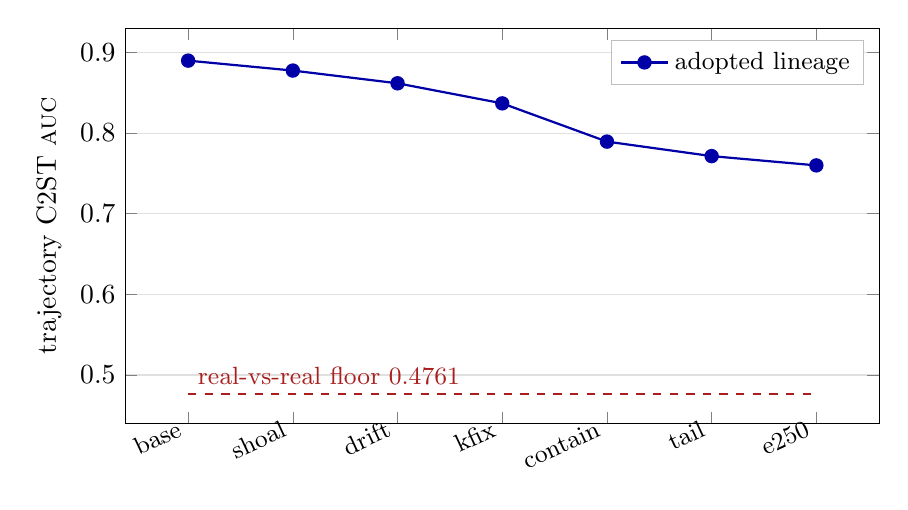
\begin{tikzpicture}
\begin{axis}[
  width=0.92\textwidth, height=6.6cm,
  ylabel={trajectory \ctst\ \auc},
  ymin=0.44, ymax=0.93,
  symbolic x coords={base,shoal,drift,kfix,contain,tail,e250},
  xtick=data, x tick label style={rotate=25,anchor=east,font=\small},
  ymajorgrids, grid style={black!12},
  every axis plot/.append style={thick},
  legend style={at={(0.98,0.97)},anchor=north east,font=\small,draw=black!25},
]
\addplot[color=blue!65!black,mark=*,mark size=2.2pt] coordinates {
  (base,0.8898) (shoal,0.8775) (drift,0.8617) (kfix,0.8368)
  (contain,0.7894) (tail,0.7714) (e250,0.7599)};
\addlegendentry{adopted lineage}
\addplot[color=losec,dashed,no marks,domain=0:1,forget plot] coordinates {(base,0.4761) (e250,0.4761)};
\node[anchor=south west,font=\small,text=losec] at (axis cs:base,0.4761) {real-vs-real floor $0.4761$};
\end{axis}
\end{tikzpicture}
\caption{The adopted lineage. Each point is that ladder's winning rung; the drop between
consecutive points is \emph{not} a paired measurement (controls are refit per ladder), but
the paired deltas in the master table are. Roughly 31\% of the closable gap has been
removed.}
\end{figure}

\paragraph{And the reported likelihood barely moves.}
Across all 24 rows, \code{bits\_per\_bout} spans $7.7329$--$7.7412$: a total range of
$\mathbf{0.0084}$ bits while the trajectory \auc\ moves $0.16$. Within the \code{kin},
\code{disp} and \code{contain} ladders it is \emph{identical} to seven digits across
rungs, because every rung of those three is a generation-time calibration applied to the
same fitted network. Two further reasons it cannot move: \code{tail} changes only the
\emph{kinematic} heads, which Metric~A does not evaluate at all, and the whole quantity is
just the first of three terms in the objective the network is actually trained on
(Eq.~\eqref{eq:joint}). Do not read this column as a model ranking. Read
\S\ref{sec:twoobjects} instead.

% =====================================================================
\section{What did not work, and why}\label{sec:negatives}
% =====================================================================

There are more entries here than in \S\ref{sec:lineage}, and several were more
informative than the successes. Three of the four most expensive were \emph{method}
errors, not modelling errors.

\subsection{Mechanism failures}

\begin{center}\small
\renewcommand{\arraystretch}{1.25}
\begin{tabular}{p{0.20\textwidth}p{0.10\textwidth}p{0.60\textwidth}}
\toprule
\textbf{mechanism} & \textbf{$\Delta$ \auc} & \textbf{diagnosis} \\
\midrule
monotone proximity (\code{dot}) & $+0.0112$ &
Cannot represent an inverted-U or a sign change. Resolvedly \emph{worse} than the
bearing-only ablation it was meant to improve. \\
border basis (\code{\_wall}) & $-0.0065$ (null) &
Fixed the conditional turn probability at the wall; occupancy is a stationary property
and did not move. \\
reflecting wall & --- &
Mechanically correct (preserves the step marginal, leaves the fish heading inward) and
metric-invisible on its own. Retained inside \code{contain}. \\
constant centre bias & --- &
Attacks entry rate only; leaves $P(r/R{>}0.85)$ at $0.033$ vs $0.012$ because the tail is
dwell. Superseded by the shell gate. \\
2-D containment & --- &
Decoupling bulk and shell scored $6\times$ worse on the calibration objective than the
1-D scale. \\
\code{kin\_var\_comp} & $+0.0570$, $+0.0324$ &
\textbf{Lost twice.} Symmetric log widening about a fixed centre: right variance, wrong
shape. \\
\code{vigor\_turn} & $+0.0480$ &
Scaling $|\dth|$ per trajectory wrecks the pooled turn marginal,
\code{abs\_dtheta\_w1} $6.67 \to 8.43$. \\
far-field knot (\code{shoalf}) & $-0.0058$ (null) &
Mechanism-positive on the restoring-force profile, undetectable on the \auc. \\
containment recalibration & $+0.0009$ (null) &
Corrected estimator, no measurable effect. \\
quantile map (\code{qmap}) & --- &
Right \emph{shape} of correction (monotone, cannot leave the support), but context-blind
and afflicted by the same fixed-point problem as the vigor drift: it is calibrated against
a rollout it then changes. \\
rollout-aware policy gradient & --- &
Density-ratio REINFORCE with an MLE anchor. A control with the policy-gradient weight set
to zero reproduced most of the gain, so the improvement was \textbf{under-training}, not
the reinforcement signal. \\
\bottomrule
\end{tabular}
\end{center}

\subsection{Method failures --- the expensive ones}

\paragraph{Oracle support violation (twice).}
An affine rescale, then a Gaussian offset, applied to \emph{bounded} window features ---
\code{rad\_frac\_wall}, \code{uni\_F}, the transition probabilities, all fractions that are
frequently exactly $0$. Both pushed values negative, outside the real support, and the
classifier detected the impossible values rather than the intended effect: \auc\ $0.997$
and $0.968$. The fix is a quantile or rank map, which preserves the support by
construction. \emph{Any oracle applied to a bounded feature must be support-preserving.}

\paragraph{The 3-fish evaluation trap (three times).}
Radial and dispersion population statistics vary 7--12$\times$ across fish. A 3-fish test
made the vigor drift fix look like a regression, and nearly caused a working containment
fix to be discarded. Between-fish spread is precisely the quantity being estimated in
these cases, so a small subset's estimate of it is worthless. This is now a written rule:
\textbf{never evaluate a dispersion, radial or individuality quantity on a 3-fish subset}.

\paragraph{Calibrating against a moving baseline (recurring).}
The vigor drift was sized so the injected drift alone carried the full real
variance --- but the rollout already varies and the two add ($1.80\times$ real). The
quantile map has the same structure: it is fitted against a rollout that the map then
alters. The general fix is to measure the baseline with the mechanism switched off, and
size the mechanism to the \emph{difference}.

\paragraph{A shared random-number stream.}
Threading one generator through the whole evaluation made every model's draws depend on
which other models were in the run and on $R$. The same configuration scored $0.760$ and
$0.7946$ purely from list composition. Fixed by per-unit streams keyed
$(\text{seed}, \text{fish}, \text{replicate})$, which additionally makes replicates
\emph{paired} across models.

\paragraph{Unnormalised multi-objective calibration.}
Summing relative errors let a $\sim$1\% occupancy dominate a $\sim$0.5 mean by $115{:}1$,
so the guard objective was inert and the search ran to the grid ceiling --- producing a
worse absolute error than doing nothing. Score competing objectives in a common,
meaningful unit (here, between-fish standard deviations), then weight by measured
importance.

\subsection{The finding that reframes the nulls}\label{sec:masking}

The \auc\ is a \emph{rank} statistic, and defects combine sub-additively. Injecting
defects into real windows one at a time gives a masking curve: an identical cross-channel
coupling defect is worth
\begin{center}
$\mathbf{+0.042}$ alone \quad$\to$\quad $\mathbf{+0.001}$ once a single 20\% marginal error
is also present \quad$\to$\quad $\mathbf{+0.049}$ again after the marginals are repaired,
\end{center}
a \textbf{40$\times$ swing} at baseline $0.740$ --- nowhere near an \auc\ ceiling.

\begin{takeaway}
A fix can measure as a clean null purely because a larger unrelated defect is absorbing
the classifier's power. \textbf{\code{far}, \code{cal}, and the turn-direction persistence
mechanism may be masked, not refuted}, and cannot be re-read until the distance marginal
is repaired --- currently \code{dist\_std} $5.84$ against a real $8.39$, i.e.\ 26--32\%
low. Never record a null as a refutation without checking what else is broken.
\end{takeaway}

\subsection{Calibrating the scale: how much structure is $0.76$?}

A block-bootstrap ladder of surrogates --- real bouts resampled in contiguous blocks of
length $L$, so the marginals are exact and $L$ bouts of temporal structure are preserved
--- places the \auc\ on an interpretable axis:
\begin{center}\small
\begin{tabular}{lrrrr}
\toprule
$L$ (bouts) & 3 & 10 & 30 & floor \\
\midrule
\auc{} & $0.674$ & $0.595$ & $0.521$ & $0.504$ \\
\bottomrule
\end{tabular}
\end{center}
Against this, the model sits at an equivalent of $\approx 2.8$ bouts of preserved
structure --- \emph{after} rank-equalising marginals. The raw placement is meaningless
because the bootstrap has exact marginals by construction and the model does not.

Two caveats. The pooled variant of this ladder is invalid: past $L=30$ it inverts
($0.226$ at $L=60$) because the surrogate is built from training fish. And the code that
produced these numbers is not in the repository, so they are reported as a measured
calibration rather than something a reader can currently regenerate.

% =====================================================================
\section{Two objects, one likelihood}\label{sec:twoobjects}
% =====================================================================

This section is the honest caveat on everything above, and it should be read before any
of the results are quoted elsewhere.

\begin{keybox}{The central fact}
The model's \code{score()} method --- the one Metric~A evaluates --- \textbf{never reads}
\code{vigor}, \code{kin\_feedback}, \code{centre\_bias}, \code{qmap}, \code{artr}, or
\code{kin\_var\_scale}. Those six live only inside the closed-loop generator. It does not
read the distance or interval heads either, even though those are fitted
(\S\ref{sec:joint}).
\textbf{Metric~A scores one object; every trajectory ever rendered comes from another.}
\end{keybox}

There is a sharper version of this, which follows from the emission definitions in
\S\ref{sec:joint}. The sampler does not merely add mechanisms on top of the fitted density
--- it \textbf{clips} the drawn travel and interval at the train-fold $q_{99.9}$ and then
\emph{rescales} them (\code{qmap}, \code{kin\_var\_scale}), in neither case renormalising.
So the law the sampler actually realises is not the density
Eqs.~\eqref{eq:pdist}--\eqref{eq:pdt} define, and it is not a normalised density at all.
The two objects are not two parameterisations of one model; only one of them is a
probability model.

Concretely: the shipped sampler discards 48\% of its own distance history
($\lambda_{\mathrm{dist}} = 0.521$) at \emph{zero} cost to the \emph{reported} likelihood.
Every ladder win from \code{kin} through \code{contain} was a win on the unfitted object,
adjudicated only by a random forest; \code{tail} changed a fitted head that Metric~A still
cannot see; and \code{conv} is the only win after \code{shoal} that the reported likelihood
could in principle have adjudicated. That search has no natural stopping criterion, which
is the real reason the ``find the largest tell, fix it, measure'' loop eventually exhausts
itself.

Because ``in the likelihood'' is ambiguous once the training objective is joint
(\S\ref{sec:joint}), the table below splits it: \emph{fitted} means the mechanism's
parameters are estimated by maximum likelihood; \emph{scored} means Metric~A can see it.
Two rows differ, and they are the two that matter.

\begin{center}\small
\renewcommand{\arraystretch}{1.15}
\begin{tabular}{@{}>{\raggedright\arraybackslash}p{0.225\textwidth}cc
                  >{\raggedright\arraybackslash}p{0.155\textwidth}
                  >{\raggedright\arraybackslash}p{0.225\textwidth}@{}}
\toprule
\textbf{mechanism} & \textbf{fitted} & \textbf{scored}
  & \textbf{dims added} & \textbf{where it lives} \\
\midrule
5-component emission & \win{yes} & \win{yes} & 0 (head $8\to14$) & network head \\
\code{shoal} range basis & \win{yes} & \win{yes} & $+15$ & input features \\
border basis & \win{yes} & \win{yes} & $+6$ & input features \\
adaptation block & \win{yes} & \win{yes} & $+2$ & input features \\
kinematic trunk + heads & \win{yes} & \lose{\textbf{no}} & $2K_{\mathrm{kin}}$ & separate trunk \\
tail components & \win{yes} & \lose{\textbf{no}} & 0 & network heads \\
convergence budget & \win{yes} & \win{yes} & 0 & training \\
\midrule
\code{vigor} intercept + drift & \lose{no} & \lose{no} & 0 & generation \\
drift re-sizing & \lose{no} & \lose{no} & 0 & generation, post-fit \\
\code{kin\_feedback} shrinkage & \lose{no} & \lose{no} & 0 & generation, post-fit \\
\code{kin\_var\_scale} & \lose{no} & \lose{no} & 0 & generation, post-fit \\
containment bias & \lose{no} & \lose{no} & 0 & generation, post-fit \\
wall mode (clip / reflect) & \lose{no} & \lose{no} & 0 & generation \\
turn-persistence oscillator & \lose{no} & \lose{no} & 0 & generation, post-fit \\
quantile map & \lose{no} & \lose{no} & 0 & generation, post-fit \\
\bottomrule
\end{tabular}
\end{center}

\noindent\small
The two mismatched rows are the sharpest statement of the problem in this section: the
kinematic trunk and its distance/interval heads, and the heavy-tailed components added to
them, are fitted by maximum likelihood inside Eq.~\eqref{eq:joint} --- and yet
\code{score()} evaluates only the angle mixture, so \textbf{neither can move
\code{bits\_per\_bout} by a single digit}. Roughly two-thirds of the fitted emission is
optimised against a likelihood that is never reported.\normalsize

\subsection{Why this is defensible, and where it is not}

In favour: every generation-only constant is calibrated on \emph{training fish only}, so
nothing leaks and the mechanisms generalise to held-out fish exactly as a fitted parameter
would. Several are provably corrective rather than cosmetic --- the between-fish variance
the vigor intercept restores is entirely in a residual the trunk cannot see, and the
exposure-bias shrinkage repairs a mismatch that exists \emph{because} training is
teacher-forced and generation is not.

Against, and these are real: (i) they are invisible to any likelihood, so only a noisy
\auc\ can adjudicate them; (ii) they are fitted \emph{sequentially}, so each absorbs the
previous ones' residuals; and (iii) \S\ref{sec:disp} and \S\ref{sec:contain} together
prove they can buy a metric win by degrading an unmeasured property. They are kept, but
instrumented (\S\ref{sec:guards}) and re-fitted in a controlled order.

\subsection{The calibration order, and the two constraints that are load-bearing}

\begin{center}
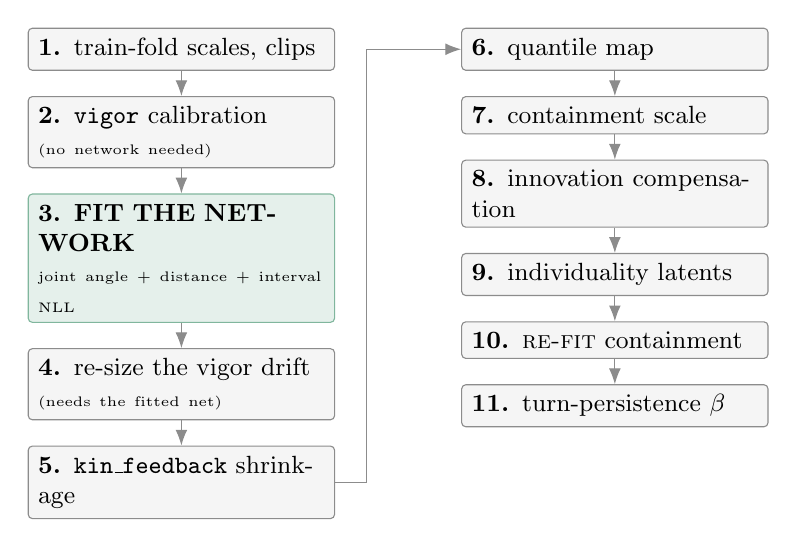
\begin{tikzpicture}[
  node distance=3.2mm,
  box/.style={draw=black!45,rounded corners=1.5pt,inner sep=3.6pt,font=\small,
              text width=0.30\textwidth,align=left},
  fitbox/.style={box,fill=winc!10,draw=winc!50},
  genbox/.style={box,fill=black!4},
  arr/.style={-{Latex[length=2mm]},draw=black!45},
]
\node[genbox] (a) {\textbf{1.} train-fold scales, clips};
\node[genbox,below=of a] (b) {\textbf{2.} \code{vigor} calibration \\ \tiny(no network needed)};
\node[fitbox,below=of b] (c) {\textbf{3. FIT THE NETWORK} \\ \tiny joint angle + distance + interval NLL};
\node[genbox,below=of c] (d) {\textbf{4.} re-size the vigor drift \\ \tiny(needs the fitted net)};
\node[genbox,below=of d] (e) {\textbf{5.} \code{kin\_feedback} shrinkage};

\node[genbox,right=16mm of a] (f) {\textbf{6.} quantile map};
\node[genbox,below=of f] (g) {\textbf{7.} containment scale};
\node[genbox,below=of g] (h) {\textbf{8.} innovation compensation};
\node[genbox,below=of h] (i) {\textbf{9.} individuality latents};
\node[genbox,below=of i] (j) {\textbf{10.} \textsc{re-fit} containment};
\node[genbox,below=of j] (k) {\textbf{11.} turn-persistence $\beta$};

\draw[arr] (a)--(b); \draw[arr] (b)--(c); \draw[arr] (c)--(d); \draw[arr] (d)--(e);
\draw[arr] (e.east) -- ++(4mm,0) |- (f.west);
\draw[arr] (f)--(g); \draw[arr] (g)--(h); \draw[arr] (h)--(i); \draw[arr] (i)--(j);
\draw[arr] (j)--(k);
\end{tikzpicture}
\end{center}

Two orderings are not cosmetic. The quantile map must precede containment, because the map
rescales step length and the wall bias has to be calibrated against the \emph{mapped}
rollout. And containment must be \textbf{re-fitted after} any mechanism that widens
movement, because movement spread drives wall contact (measured correlation $+0.59$) and
wall occupancy is the single largest \ctst\ feature --- omitting that re-fit is exactly how
\code{contain\_vc} lost. One asymmetry remains unresolved: the turn-persistence
calibration runs last, after three mechanisms have changed the turn stream, and the
quantile map is never re-fitted after a later mechanism widens the marginals it was
matched to.

% =====================================================================
\section{Where the model stands}\label{sec:standing}
% =====================================================================

\subsection{Dispersion}

\begin{center}\small
\begin{tabular}{lrrrrrr}
\toprule
& turn & distance & interval & dot-dist & radial & \textbf{between-fish share} \\
\midrule
\code{shoal} (start)   & $0.71$ & $1.23$ & $0.55$ & $1.18$ & $2.17$ & $0.063$ \\
\code{shoal\_kfix}     & $0.69$ & $0.52$ & $0.34$ & $1.16$ & $1.98$ & $0.078$ \\
\code{contain}         & $0.69$ & $0.51$ & $0.33$ & $0.94$ & $0.72$ & $0.083$ \\
\code{e250} (current)  & $0.68$ & \lose{$0.51$} & \lose{$0.40$} & $0.96$ & $0.65$ & \lose{$0.081$} \\
\midrule
\textit{real target}   & $1.00$ & $1.00$ & $1.00$ & $1.00$ & $1.00$ & $\mathbf{0.255}$ \\
\bottomrule
\end{tabular}
\end{center}

\begin{figure}[h]\centering
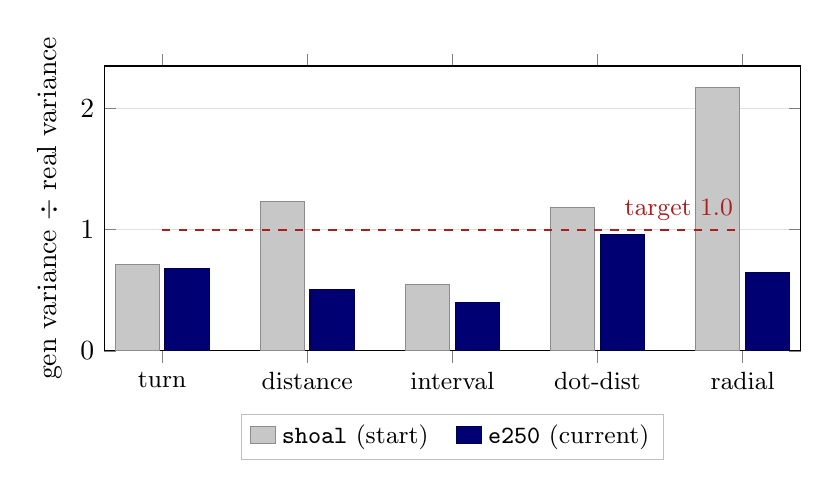
\begin{tikzpicture}
\begin{axis}[
  width=0.86\textwidth, height=5.2cm,
  ybar, bar width=16pt,
  ylabel={gen variance $\div$ real variance},
  ymin=0, ymax=2.35,
  symbolic x coords={turn,distance,interval,dot-dist,radial},
  xtick=data, x tick label style={font=\small},
  ymajorgrids, grid style={black!12},
  legend style={at={(0.5,-0.22)},anchor=north,legend columns=2,font=\small,
                draw=black!25,/tikz/every even column/.append style={column sep=8pt}},
  % default ybar legend marks are thin slivers; draw proper swatches instead
  legend image code/.code={\draw[#1] (0cm,-0.09cm) rectangle (0.32cm,0.13cm);},
]
\addplot[fill=black!22,draw=black!45] coordinates {
  (turn,0.71) (distance,1.23) (interval,0.55) (dot-dist,1.18) (radial,2.17)};
\addlegendentry{\code{shoal} (start)}
\addplot[fill=blue!45!black,draw=blue!30!black] coordinates {
  (turn,0.68) (distance,0.51) (interval,0.40) (dot-dist,0.96) (radial,0.65)};
\addlegendentry{\code{e250} (current)}
\draw[losec,thick,dashed] (axis cs:turn,1) -- (axis cs:radial,1);
\node[anchor=south east,font=\small,text=losec] at (axis cs:radial,1.0) {target $1.0$};
\end{axis}
\end{tikzpicture}
\caption{Radial over-dispersion was eliminated ($2.17 \to 0.65$, slightly overshooting) and
dot-distance brought to target. The behavioural channels remain \emph{under}-dispersed:
the model is still too typical.}
\end{figure}

\subsection{The three honest deficits}

\paragraph{1. Individuality.} The between-fish variance share sits at $0.081$ against a
real $0.255$ and has barely moved in nine experiments --- not because the mechanism is
mistuned but because \textbf{there is no mechanism}. The vigor latent covers interval and
distance \emph{level} only, and its turn term is hard-set to zero. Measured consequence:
the between-fish spread of forward fraction is $0.005$ generated against $0.054$ real, and
of median $|\dth|$ is 0.6\dg{} against 6.7\dg. Every generated fish
turns like the average fish. This is now the largest single identifiable gap.

\paragraph{2. Under-dispersion of the behavioural channels.} Distance sits at $0.51$ and
interval at $0.40$ against a target of $1.0$, and the cause is precisely located: a scalar
shrinkage on the kinematic history couples autocorrelation and spread through the
stationary variance $\sigma^2/(1-\varphi^2)$, so one gets the correct lag-1 \emph{or} the
correct spread, not both.

\paragraph{3. Timing.} Quiescent time is 6.4\% of the session against a real 24.4\%,
the clock ratio is $0.81$, and the bout-rate autocorrelation at 1/2/3 minutes is
$0.24/0.05/0.00$ against $0.51/0.33/0.22$. The cause is a missing right tail in the
interval distribution, not missing slow correlation --- $P(\mathrm{d}t > 20\uu{s})$
is $0.006$--$0.008$ against $0.011$.

\subsection{Final panel, current model}

\begin{center}\small
\begin{tabular}{lrrl}
\toprule
& \code{dotb} (start) & \code{e250} (current) & target \\
\midrule
trajectory \ctst\ \auc{} & $0.8898$ & $\mathbf{0.7599}$ & $0.4761$ \\
turn \ctst\ \auc{} & $0.5981$ & $0.5875$ & $\approx 0.5$ \\
\code{bits\_per\_bout} & $7.7406$ & $7.7395$ & lower \\
\code{abs\_dtheta\_w1} (deg) & $6.90$ & $6.75$ & $0$ \\
\code{dist\_w1} (px) & $3.21$ & $3.30$ & $0$ \\
\code{dt\_w1} (s) & $0.881$ & $0.885$ & $0$ \\
\code{dot\_dist\_bias\_late} (px) & $+6.96$ & $-2.79$ & $0$ \\
\code{wall\_frac\_gap} & $0.0667$ & $\mathbf{0.0019}$ & $0$ \\
\bottomrule
\end{tabular}
\end{center}

Note that the two channels that improved dramatically --- shoal distance and wall
occupancy --- are the two that were structurally broken, while the three per-bout marginal
distances are essentially unchanged. That is the correct reading of what nine experiments
bought: \textbf{the trajectory-level geometry was repaired; the per-bout marginals were
already close and remain so.}

% =====================================================================
\section{Next steps}\label{sec:next}
% =====================================================================

Two further experiments were built after this document's cut-off and are named here for
completeness, without results:

\begin{description}\itemsep3pt
\item[\code{mem}] A four-arm memory and attribution ladder. The shrinkage exists only to
      suppress a lag-1 overshoot that may itself be an artefact of a 3-lag history --- with
      three lags you cannot obtain a slow tail without inflating the head. The ladder
      includes a no-shrinkage control, because otherwise a longer-history win would be
      miscredited to the memory. Free-run stability sets a hard ceiling at
      $K_{\mathrm{kin}} = 8$: longer histories diverge in a substantial fraction of
      initialisations, and the validation loss cannot see it.
\item[\code{indiv}] Two per-trajectory latents for the channels the vigor latent never
      covered: \emph{turning style}, by tilting the forward mixture weight rather than
      scaling $|\dth|$ --- scaling is exactly how \code{vigor\_turn} failed --- and
      \emph{spatial preference}, by multiplying rather than offsetting the containment
      bias, since an additive offset leaks straight into the turn marginal. Both widen
      movement, so the fit re-runs the containment calibration afterwards.
\end{description}

Beyond those, the two well-posed open problems are: a variance-compensated shrinkage that
rescales the autoregressive \emph{innovation} rather than the emitted value, decoupling
autocorrelation from spread; and a slow latent state scoped to the \emph{timing} channel
only, which is where the residual slow structure demonstrably lives.

\appendix
% =====================================================================
\section{Constants and hyperparameters}
% =====================================================================

\begin{center}\small
\begin{tabular}{llp{0.42\textwidth}}
\toprule
\textbf{symbol} & \textbf{value} & \textbf{meaning} \\
\midrule
\multicolumn{3}{l}{\textit{Segmentation}}\\
\code{FPS} & $30$ & frame rate \\
\code{PX\_PER\_MM} & $3.67$ & projector scale (pixel-native pipeline) \\
smoothing $\sigma$ & 2 frames & detection only; kinematics use raw positions \\
refractory & 0.4\uu{s} & minimum inter-bout separation \\
displacement gate & $0.3$--18\uu{mm} & over $\pm0.5\uu{s}$ \\
forward threshold & 10\dg{} & $|\dth| < 10^\circ \Rightarrow$ forward \\
\midrule
\multicolumn{3}{l}{\textit{Network}}\\
$K$ & 8 & angle history lags \\
hidden & 128 & angle trunk width \\
$K_{\mathrm{kin}}$ & 3 & kinematic history lags \\
kin hidden & 32 & kinematic trunk width \\
$n_{\mathrm{dist}}, n_{\mathrm{dt}}$ & $2, 3$ & log-normal mixture components (after \code{tail}) \\
optimiser & Adam & lr $10^{-3}$, wd $10^{-5}$ (kin trunk $10^{-4}$) \\
epochs / patience & 250 / 30 & after \code{conv}; previously 80 / 8 \\
\midrule
\multicolumn{3}{l}{\textit{Shoal basis}}\\
knots & $25, 50, 90, 160\uu{px}$ & softmax basis over $\log r$ \\
width & $0.40$ & natural-log units \\
$r_{\mathrm{ref}}$, octave & $70\uu{px}$, $\log 4$ & $r_z$ pivot and scale \\
\midrule
\multicolumn{3}{l}{\textit{Border basis}}\\
knots & $0.03, 0.10, 0.25, 0.55$ & in $d_{\mathrm{norm}}$ ($0 =$ wall) \\
width & $0.55$ & natural-log units \\
\midrule
\multicolumn{3}{l}{\textit{Containment}}\\
$u_0$ & $0.75$ & shell gate threshold in $r/R$ \\
base $(\mathrm{bulk},\mathrm{shell})$ & $(4^\circ, 35^\circ)$ & scaled by a fitted $s \in [0,3]$ \\
$w_{\mathrm{occ}}$ & $2.6$ & occupancy weight vs mean radius \\
calibration fish & 12 & never fewer --- see \S\ref{sec:negatives} \\
\midrule
\multicolumn{3}{l}{\textit{Evaluation}}\\
folds & 5 & leave-3-fish-out \\
$R$ & 12 & panel rollouts per held-out fish \\
\ctst\ replicates & 8 & $t_{\mathrm{crit}} = 2.3646$ \\
window $W$ & 60 bouts & non-overlapping \\
classifier & RF(200) & GroupKFold by fish \\
floor & $0.4761$ & real-vs-real negative control \\
\bottomrule
\end{tabular}
\end{center}

% =====================================================================
\section{Naming grammar}
% =====================================================================

Every result is labelled by a token string, read left to right as a stack of
modifications on the base model:

\begin{center}\small
\begin{tabular}{@{}>{\raggedright\arraybackslash}p{0.30\textwidth}
                  >{\raggedright\arraybackslash}p{0.62\textwidth}@{}}
\toprule
\textbf{token} & \textbf{meaning} \\
\midrule
\code{mlp}, \code{full} & feed-forward MDN, per-bout parameter head \\
\code{border} & border feature block present \\
\code{h128} & hidden width 128 (and $K = 8$) \\
\code{mix} & 5-component angle emission (14 outputs) \\
\code{dotb} / \code{dot} / \code{shoalr} / \code{shoal} / \code{shoalf} & stimulus mode: 3 / 6 / 13 / 18 / 21 channels \\
\code{wall} & border \emph{basis} (9 channels) instead of raw (3) \\
\code{loop} / \code{guard} / \code{hloop} & closed loop / guardrail only / \textbf{honest} loop (stimulus also recomputed) \\
\code{kin} & separate kinematic trunk with autoregressive distance and interval \\
\code{vigor}, \code{turn} & per-trajectory latents (level; magnitude) \\
\code{drift} & vigor drift re-sizing \\
\code{kfix} & kinematic feedback shrinkage \\
\code{vc} & variance compensation (rejected) \\
\code{contain} & shell-gated containment bias (implies reflecting wall) \\
\code{tail} & $n_{\mathrm{dist}} = 2$, $n_{\mathrm{dt}} = 3$ \\
\code{artr} & slow left/right turn-bias oscillator \\
\code{e250} & 250 epochs, patience 30 \\
\bottomrule
\end{tabular}
\end{center}

So \code{mlp\_border\_full\_h128\_mix\_shoal\_hloop\_kin\_vigor\_contain\_tail} --- the
model this document ends at, before the epoch change --- is: a feed-forward MDN with a
border block, per-bout parameters, width 128 with 8 angle lags, a 5-component emission,
the 18-channel shoal stimulus, an honest closed loop, a separate kinematic trunk with
per-trajectory vigor latents, shell-gated containment, and heavy-tailed kinematic heads.

% =====================================================================
\section{Reproduction}
% =====================================================================

Training and evaluation run on a single A100 via a reproducible bundle. Local:
\begin{center}\code{python make\_colab\_bundle.py}\quad(or \code{--check} to verify the zip
matches the working tree)\end{center}
which packages the scripts, the bout table, the physical dish ROI and the notebook, but
deliberately excludes the transformed per-frame trajectories --- they are needed only for
video rendering, which is done locally. Remote:
\begin{center}\code{python colab\_run\_ladder.py --ladder \{stim,wall,kin,disp,contain,tail,far,cal,conv\}}\end{center}
Each invocation fits every rung of that ladder inside one run under common random numbers
and writes \code{ladder\_\{name\}\_results.zip} containing \code{results.csv} (the panel and
both \auc{} s), \code{panel.csv} (per-fish, including the guards), \code{likA.csv}, and
\code{artifacts.pkl} (the per-replicate \auc\ vectors that every paired contrast in this
document is computed from), alongside the fitted checkpoints. Wall-clock is roughly 1--6
hours depending on the number of rungs.

% =====================================================================
\section{Provenance, and known documentation defects}
% =====================================================================

\paragraph{Where these numbers come from.} Every figure in \S\ref{sec:lineage} and
\S\ref{sec:standing} is read from the nine ladder result archives. \textbf{The
\code{results.csv} / \code{panel.csv} / \code{artifacts.pkl} at the repository root are
not results} --- they are a smoke run (2 folds, $R=2$, 3 epochs) whose rung names match the
first ladder but whose \auc{} s do not. They are easy to pick up by mistake.

\paragraph{Column that should not be tabulated.} \code{density\_skill\_bits} is all-NaN in
every row of every ladder.

\paragraph{Disagreements between the existing \texttt{methods.tex} and the code or data,
which should be reconciled if the two documents are merged:}
\begin{enumerate}\itemsep2pt
\item Stimulus speed is given in \unit{mm/s} in \code{methods.tex} and in
      \unit{cm/s} in the data overview. The label value is $3.5$ either
      way; one of the two units is wrong.
\item Group sizes: the data overview omits $N=1$, but labels \code{g0-1} and \code{g1-0}
      exist in the bout table. \code{methods.tex} is correct.
\item \code{methods.tex} describes a per-dish millimetre rescaling. The current pipeline is
      pixel-native and performs no such rescaling; that passage is stale.
\item \code{methods.tex} has \textbf{no evaluation section at all} --- it stops at the
      input-driven HMM. Sections \ref{sec:eval} and \ref{sec:twoobjects} of this document
      have no counterpart there.
\item A docstring in \code{generative\_metrics.py} states that the random-number stream key
      includes the model index; its own next paragraph and the code say the opposite. The
      code is authoritative: the model is deliberately excluded, which is what makes
      replicates paired across models.
\end{enumerate}

\paragraph{Not currently reproducible.} The block-bootstrap calibration in
\S\ref{sec:negatives} was measured, but its generating code is not in the repository.

\end{document}
